%% LaTeX template for BSc Computing for Games final year project dissertations
%% by Edward Powley
%% Games Academy, Falmouth University, UK

%% Based on:
%% bare_jrnl.tex
%% V1.4b
%% 2015/08/26
%% by Michael Shell
%% see http://www.michaelshell.org/
%% for current contact information.
%%
%% This is a skeleton file demonstrating the use of IEEEtran.cls
%% (requires IEEEtran.cls version 1.8b or later) with an IEEE
%% journal paper.
%%
%% Support sites:
%% http://www.michaelshell.org/tex/ieeetran/
%% http://www.ctan.org/pkg/ieeetran
%% and
%% http://www.ieee.org/

%%*************************************************************************
%% Legal Notice:
%% This code is offered as-is without any warranty either expressed or
%% implied; without even the implied warranty of MERCHANTABILITY or
%% FITNESS FOR A PARTICULAR PURPOSE! 
%% User assumes all risk.
%% In no event shall the IEEE or any contributor to this code be liable for
%% any damages or losses, including, but not limited to, incidental,
%% consequential, or any other damages, resulting from the use or misuse
%% of any information contained here.
%%
%% All comments are the opinions of their respective authors and are not
%% necessarily endorsed by the IEEE.
%%
%% This work is distributed under the LaTeX Project Public License (LPPL)
%% ( http://www.latex-project.org/ ) version 1.3, and may be freely used,
%% distributed and modified. A copy of the LPPL, version 1.3, is included
%% in the base LaTeX documentation of all distributions of LaTeX released
%% 2003/12/01 or later.
%% Retain all contribution notices and credits.
%% ** Modified files should be clearly indicated as such, including  **
%% ** renaming them and changing author support contact information. **
%%*************************************************************************


\documentclass[journal]{IEEEtran}

\usepackage{graphicx}
% Insert additional usepackage commands here
\usepackage{hyperref}

\usepackage{listings}

\renewcommand\textminus{-}

\begin{document}
%
% paper title
% Titles are generally capitalized except for words such as a, an, and, as,
% at, but, by, for, in, nor, of, on, or, the, to and up, which are usually
% not capitalized unless they are the first or last word of the title.
% Linebreaks \\ can be used within to get better formatting as desired.
% Do not put math or special symbols in the title.
\title{How is Player Enjoyment and Challenge Affected When Implementing Dynamic Difficulty into a Top-Down Shooter?}
%
%
% author name
\author{Adrian Carter - 1703170}

% The paper headers -- please do not change these, but uncomment one of them as appropriate
% Uncomment this one for COMP320
% \markboth{COMP320: Research Review and Proposal}{COMP320: Research Review and Proposal}
% Uncomment this one for COMP360
\markboth{COMP360: Dissertation}{COMP360: Dissertation}

% make the title area
\maketitle

% As a general rule, do not put math, special symbols or citations
% in the abstract or keywords.
\begin{abstract}
With the rapid growth of the video games industry and its popularity, players are more varied and diverse than ever before. With this diversity comes a plethora of problems for game developers. One such problem is the effectiveness of static difficulty settings. Static difficulty settings have been standard in most mainstream commercial games. However more and more research is being conducted with dynamic difficulty adjustment systems that can adjust difficulty settings during runtime. This study aims to test the effect on perceived player experience of a dynamic difficulty system when compared to a static difficulty system. Specifically within the context of a singleplayer, top down shooter level with an average play time of under 3 minutes. Effectiveness is measured based on player experience feedback using questionnaires and telemetry data during gameplay.

\end{abstract}

\section{Introduction}
% The very first letter is a 2 line initial drop letter followed
% by the rest of the first word in caps.
% 
% form to use if the first word consists of a single letter:
% \IEEEPARstart{A}{demo} file is ....
% 
% form to use if you need the single drop letter followed by
% normal text (unknown if ever used by the IEEE):
% \IEEEPARstart{A}{}demo file is ....
% 
% Some journals put the first two words in caps:
% \IEEEPARstart{T}{his demo} file is ....
% 
% Here we have the typical use of a "T" for an initial drop letter
% and "HIS" in caps to complete the first word.
\IEEEPARstart{T}{his} research project investigates the effects Dynamic Difficulty Adjustment (DDA) can have on Player Experience, specifically the effect on Player Enjoyment and Challenge perception. With a more diverse variety of people playing video games than ever before \cite{juul2010casual} more care has to be taken when designing difficulty in video games. However, with the advancements of computational systems, it is becoming easier for developers to manage and adjust a wide variety of parameters in video games, even while the game is running. This has led to the expansion of DDA in recent years, enabling the designer to have more control over different difficulty factors. To adjust the difficulty, many heuristics can be considered. Heuristics ranging from affective feedback \cite{liu2009dynamic} to player performance \cite{denisova2015adaptation}. These heuristics are discussed in this paper in order to select appropriate methods that might be utilized in the creation of a bespoke dynamic difficulty system. This paper hypothesises that if one were to create two difficulty settings for a 2D top down shooter, one static and the other dynamic, the dynamic setting will be preferred by players. The paper also hypothesizes that the dynamic setting will have less variation in challenge for players, since the dynamic setting should adapt better to players of varying skill levels.
Section II of the paper will look at some of the theories and concepts that are relevant to the research question. The most prominent aspects that need to be considered when designing a dynamic difficulty system include player experience, flow theory, and player modelling. Section III discusses some of the most notable implementations of dynamic difficulty and why some of those techniques would be useful in designing a dynamic difficulty system for a 2D top down shooter with short levels. Section IV will discuss the methodology by which this paper intends to answer the proposed research question and test the hypotheses. Section V explains the design of the Artefact created in order to carry out the experiment. Section VI walks through the development and testing of the Artefact. Section VII analyses the data gathered during the experiment with regards to the hypotheses. Section VIII discusses the results from the experiment in more detail.

\section{Related Work}

\subsection{Player Experience}
Player experience in games is often described using terms such as flow, immersion, engagement, fun, and presence \cite{isbister2008game} \cite{czikszentmihalyi1990flow} \cite{mcmahan2013immersion}. Measuring this is no easy task due to the subjective nature of player experience. Although tools can be used to objectively measure some quantitative aspects of the player experience such as biosensors to measure heart rates  or electrodermal activity (measure of sweat perspiration)\cite{mikami2017adaptable} \cite{ambinder2011biofeedback} \cite{liu2009dynamic}, they still require evaluation based on the subjective experiences of the individual. Questionnaires can be particularly useful in measuring the subjective experiences of players in a quantifiable manner, due to the fact they include a number of standardised tests that can be aligned with what the researcher intends to measure about said experience \cite{ijsselsteijn2013game}.

To ensure that player experience is enjoyable, the idea of Flow must be considered. Cziksentmihalyi \cite{czikszentmihalyi1990flow} \cite{csikszentmihalyi2014toward} uses the term ``Optimal Experience'' to describe the moments in which a person feels a deep sense of enjoyment or exhilaration and states that these moments are, more often than not, due to events in which that person's body or mind is stretched to its limits in an effort to achieve something difficult or challenging.
The experience of Flow, or ``Optimal Experience'', in games is the experience gamers describe when immersed in video games, becoming entranced and totally focussed on their actions and losing track of time and other worries. Whether a player enjoys a video game is largely dependent on whether that game provides a Flow experience. In Flow theory, the idea of the Flow Zone (see figure 1) is the notion that in order to maintain a players Flow experience, the game must ideally balance challenge and the ability of the player to overcome that challenge. If the game becomes too challenging, the player becomes disheartened and anxious \cite{gilleade2004using}. On the other hand, if the game becomes too easy, the player grows bored and disinterested \cite{chanel2008boredom}. The art of good game design, is therefore in the ability of the developer to balance challenge and player ability or skill for the duration of a game experience \cite{koster2013theory}. This becomes more difficult the larger the game grows and also the larger the potential audience becomes. With a larger potential audience, the fact that each person experiences activities in different ways becomes problematic for game designers. Every player is different, with varying skill levels and expects a different level of challenge in order to experience Flow \cite{czikszentmihalyi1990flow}. The most widely used solution for this problem in video games has been the implementation of various difficulty modes (Easy, Medium, Hard etc) \cite{alexander2013investigation}. One of the problems with this is the lack of detail the player is given when choosing a difficulty level. How easy is Easy? How hard is Hard? Without playing through the game, the player won't really be able to know which mode is best suited for their skills, since difficulty ratings are generally subjective \cite{qin2009effects}. This is where the notion of DDA becomes very useful to developers.

\begin{figure}[h]
	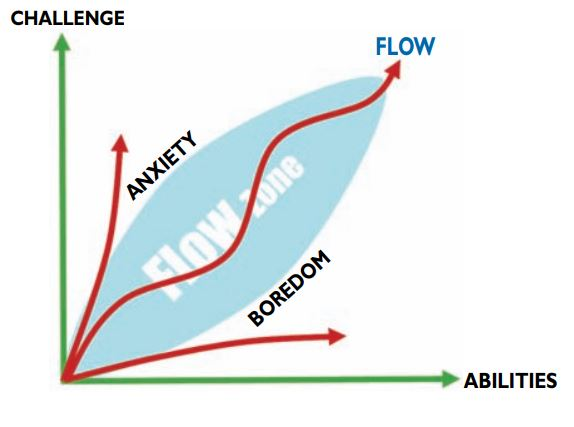
\includegraphics[width=1.0\linewidth]{FlowChart.jpg}
	\caption{Chen, Flow in Games ~\cite{Chen:2007:FG:1232743.1232769}.}
	\label{FlowChart}
\end{figure} 


\subsection{Player Experience Modelling}

While there has been much research on what constitutes fun in game design and how player engagement lends itself to other aspects of player experience \cite{salen2004rules} \cite{koster2013theory}, much of this research is qualitative in nature and serves mainly to aid in game design conceptually. Less research exists in the field regarding quantitative measurement of player experience and player modelling. The primary objective of player experience and player modelling research, is to describe how players interact with and experience a game. 

Player Experience Modelling, in the context of this paper, refers to the modelling of complex and dynamic aspects of a player interacting with the world during gameplay. Specifically the study and use of AI techniques to create computational models of player experience. This is not to be confused with player profiling, which deals with the types of players you are designing the game for \cite{bartle1996hearts}. 

Yannakakis et al \cite{yannakakis2013player} argue that one of the main aims of studying players in games is to gain an understanding of players' cognitive, affective and behavioural patterns. This is strongly related to the field of Human Computer Interaction \cite{preece1994human} \cite{fischer2001user} and usability. 

The simplest way of generating a model of player experience is to ask the players themselves and build a model based on the collected data. Yannakakis et al \cite{yannakakis2012game} describe this as Subjective Player Experience Modelling. Using short questionnaires like this seems like an effective method to model player experience during the experiment. This study \cite{pedersen2009modeling} used gameplay interactions to construct a computational model of player experience using statistical features such as how often and when the player jumped, ran, died etc. Whilst it is out of the scope of this paper to collect data such as this during development in order to adapt the dynamic algorithm design, this data collection method would be useful in measuring the effectiveness of said design once complete.

The creators of Polymorph \cite{jennings2010polymorph} used methods from machine learning and procedural content generation to create a 2D platformer that generates upcoming parts of the level based on the current skill of the player. In order to create the system, a model of difficulty was required. Instead of modelling difficulty based on subjective game design ideas, the creators designed a mass data collection tool to gather information about level segments directly from players. Each player would play a short segment of the level and then give feedback by rating the perceived difficulty on a scale from 1 to 6. The tool would also collect telemetry data on the players behaviour while playing the level segment which could be applied to a machine learning algorithm in order to model player skill. Again, there are clear differences in this study to the one in this paper, however, the collection of player behavioural data is something worth considering when testing the effectiveness of the dynamic and static difficulty settings.



\section{Dynamic Difficulty Adjustments}
The challenge of designing a difficulty curve for players of varying skill level is a big problem even experienced designers with strong domain knowledge have difficulty solving. In contrast to static difficulty, dynamic difficulty adjustment (DDA) attempts to address this issue. 
 
Currently, research in the field of DDA is in a state that does not allow for particularly complex systems, and as such, cannot be used as a framework for DDA systems in other games. Although some research is being done to establish DDA frameworks \cite{zohaib2018dynamic}, they generally cover only certain basic elements of gameplay, usually within 2D games \cite{wheat2013dynamically} and more complex variants need to be implemented in bespoke ways, depending on the genre and game elements that need to be adjusted. 

The ways in which these methods adjust difficulty may differ, but they all exhibit a common theme in prediction and intervention.

\subsection{Dynamic Scripting}
Dynamic scripting (DS) is an online learning approach that maximises an AI players chance of winning a game by determining what tactics will lead to the solution, when presented with a certain problem and domain \cite{spronck2004online}. Using dynamic scripting, the AI player adapts its tactics based on the opponents' tactics using domain-specific knowledge and several rulebases that categorize various opponent types. Each script rule is assigned a weighting value that is adjusted based on the success or failure rates of said rule.

The AI learns and adapts progressively using this technique. The AI will update the weight value of the current rules being used during a confrontation with the player, based on the outcome of said confrontation. If the resulting outcome is beneficial to the AI, the rules that lead to that outcome will have their weight values increased, whereas the rules that were counter to that outcome will have their weight values decreased. If the outcome is detrimental to the AI then the inverse occurs. Remaining rules adjust accordingly to keep the sum of all weighted values in the rulebase constant.
Eventually, the AI would become too difficult for human players to compete with and so would need to be balanced properly \cite{liden2003artificial}. In order to balance the opponents ability with the players, there are three common ways to modify dynamic scripting:

\begin{enumerate}
\item High-fitness penalizing: Increase or decrease weight values proportional to a fitness value. Reward suboptimal behaviour and penalize superior behaviour to essentially make the AI less efficient.
\item Weight clipping: Uses a maximum weight value to limit the rules that are chosen from the rulebase. The higher the maximum value the greater the disparity between the most optimal and least optimal rules. Lowering the maximum weight value during gameplay would make less optimal rules more likely to be chosen, thereby decreasing the effective difficulty of the opponent, and vice versa.
\item Weight culling: As with weight clipping, uses a maximum weight value limiter. However, the weight value of rules are allowed to extend above the maximum value. When a rule has a weight above maximum, the AI is unable to select said rule, thus automatically balancing the AI strength in proportion to the player.
\end{enumerate}

The commercial viability of this Adaptive AI has been dismissed by some developers in the past \cite{woodcock2000future} \cite{rabin2004promising}. The reason for this is the inherent difficulty in creating game AI with online learning capabilities without the fear that the AI will learn inferior behaviour. This is a large concern, particularly to publishers, in the games industry. Simple games with less computational risk have been seen to work \cite{demasi2003line} and research has been done to effectively implement Adaptive AI using DS into existing commercial games  \cite{spronck2006adaptive}.

\subsection{Resident Evil 4}
\textit{Resident Evil 4} \cite{game:re4} was created with a hidden grading system that judged the players performance in the background unbeknownst to the player. The system grades the player from 1 to 10 with higher grades leading to a higher challenge. If the player plays well by scoring headshots often and surviving for long periods without dying very often, the player is given a high grading which means more enemy spawns and more powerful enemies with higher health and better accuracy etc. If the player dies a lot or is inaccurate and generally not playing very well, the system lowers the players grade, and with that the enemies become fewer and less dangerous. The constant adjustment of difficulty without the player even knowing this system was in place, lead to a great experience for the players. Knowing that a game has dynamic difficulty adjustments in place can sometimes affect the experience for the players. In this way, a DDA system should adapt to the player in an inconspicuous manner, so the player is not aware of the outer intervention.
While the techniques in this system are bespoke to the game, the general idea of a player rating system to model ability is one that is prevalent in the field of DDA. The heuristics used would also be useful in the creation of a dynamic difficulty system.  

\subsection{Homeworld}
One example of potential abuse of a difficulty system is seen in \textit{Homeworld} \cite{game:homeworld}. The game is a space strategy simulator that involves the player collecting resources and building units to fight an AI team of similar units. At the end of a mission, the system would rate the power of your current fleet size and adjust the number of units that would be spawned when you started the next mission, effectively raising or lowering the difficulty. Unfortunately, once players realised this, they looked for ways to abuse the system by scrapping their entire fleet before ending the mission. This would make the next mission much easier since there would be fewer enemies spawned but by scrapping their fleet, they still retained the resources needed to quickly build another large and powerful fleet and ``steamroll'' the enemy AI fleet.

\subsection{Left 4 Dead AI Director}
The \textit{Left 4 Dead} games created by Valve are 4 player cooperative first-person shooter games \cite{game:left4dead} \cite{game:left4dead2}. The Artificial Intelligence (AI) director found within both \textit{Left 4 Dead} games is focussed on maintaining pace: having an intensity that peaks and troughs throughout play \cite{booth2009ai}. This intensity fluctuates in real time and alters the frequency and strength of enemy waves during a given game. This keeps players on edge throughout the game and ensures the players make progress towards an end goal. If the players stay in any one area for too long, the director sends more enemies their way to encourage them to keep moving. This method makes the game far more replayable than games with more traditional, static spawning systems due to the uniquely unpredictable enemy spawns.

In order to determine each players ``skill'' the AI director closely monitors the performance of each player. Determining a player's skill level quantitatively becomes problematic since we tend to judge skill based on qualitative measures. However, there are many attributes that could be employed to determine a players skill value in an fps: their overall health, damage ratio (received vs delivered), enemy kills, health packs used, shot accuracy, ammunition consumption rate and many more. These attributes can be used to help evaluate player skill and would be suitable heuristics to use in developing a dynamic difficulty system.

The AI director also attempts to model player emotional intensity, or ``stress'' level, throughout each game. This helps determine how intense each player is finding the game at that time. This is quantitatively measured using factors such as: enemy proximity to player, number of enemies in level, number of enemies actively attacking player, enemy proximity to player on enemy death etc. In the game, special enemies have the ability to incapacitate the player, if this happens, the emotional intensity of the player reaches it's maximum value. As well as normal enemy spawns, the director also has the ability to spawn a ``mob'' of 10 - 30 normal enemies behind or to the sides of the player route in order to surprise the player. There are limits to the number of enemies that can in the level at any one time and cooldowns to these ``mob'' spawn events so as not to completely overwhelm the players. The idea of using an emotional intensity value is very intriguing. It would be very interesting to see if this could be scaled down and adapted to suit a game with shorter levels. 

Both player ``skill'' and ``stress'' values, along with other pieces of information such as how long the player has spent in the current area, are used by the AI director to manage the pace of the game. The director will influence the pacing by controlling where enemies are spawned, how many enemies are spawned, what enemies are spawned, how enemies will act, ammo and health spawns among many other factors. For example, a typical level will start with a small number of normal enemies, increase the spawn rates of enemies gradually and introduce special enemies until the players stress levels reach a maximum value. Then, at the peak of game intensity, the AI director will cease spawning enemies and give the players a brief respite of around 30 seconds to organize themselves before moving forward.
Overall, this system to create pacing, peaks and troughs of intense gameplay would be an interesting route to go down to see if it could be adapted to suit shorter play times. 
 
\subsection{Hamlet}
\textit{Hamlet} \cite{hunicke2005case} is a DDA tool built by \textit{Hunicke and Chapman} that uses methods taken from \textit{Operations Research and Inventory Management}. The tool would adjust the difficulty of the first person shooter \textit{Half-Life} \cite{game:halflife} as the player progressed through the level. Algorithms were created to measure the difficulty based on the speed at which the player progressed and what resources the player currently had. It essentially manipulates the game difficulty by studying and adjusting the supply and demand of the players inventory.


\section{Methodology}
The philosophy underpinning this paper is largely based on Empiricism. The view that information is primarily gained through sensory experience. Hence my methodology will mainly talk about how to quantify subjective data using likert scales and using telemetry data in order to empirically evaluate the effectiveness of my computing artefact.

\begin{table*}[t]
\centering
\caption{Hypotheses Table}
\label{tab:my-table}
\begin{tabular}{|l|l|l|l|}
\hline
  & \textbf{Hypothesis}                                                                                                                                                               & \textbf{Null Hypothesis}                                                                                                                                                              & Data Source                                                                       \\ \hline
1 & \begin{tabular}[c]{@{}l@{}}Players will enjoy playing the version with dynamic\\ difficulty more than the version with static difficulty\end{tabular}                             & \begin{tabular}[c]{@{}l@{}}Players will not enjoy  playing the version with dynamic \\ difficulty more than the version with static difficulty\end{tabular}                           & Questionnaire                                                                     \\ \hline
2 & \begin{tabular}[c]{@{}l@{}}There will be more variation in how challenged\\ players were playing with static difficulty than when \\ playing with dynamic difficulty\end{tabular} & \begin{tabular}[c]{@{}l@{}}There will not be more variation in how challenged\\ players were playing with static difficulty than when \\ playing with dynamic difficulty\end{tabular} & \begin{tabular}[c]{@{}l@{}}Questionnaire\\ \\ Gameplay \\ Statistics\end{tabular} \\ \hline
3 & \begin{tabular}[c]{@{}l@{}}Players will be unable to reliably judge which \\ version used dynamic difficulty\end{tabular}                                                         & \begin{tabular}[c]{@{}l@{}}Players will be able to reliably judge which \\ version used dynamic difficulty\end{tabular}                                                               & Questionnaire                                                                     \\ \hline
\end{tabular}
\end{table*}

\subsection{Hypotheses}

When designing a dynamic difficulty system there are several objectives one can hope to achieve. One objective is to create a system that leads to increased replayability of a game. One might also wish to implement DDA to make a game more accessible to players of varying skill levels. Another aim could be to create a system that enhances overall player enjoyment. For the scope of this paper, the focus is on creating a dynamic system that is effective in a game with shorter levels. Effective can mean a variety of things, in this case an effective dynamic difficulty system would be one that is more enjoyable and engaging than that of a standard static difficulty system. Xue et al \cite{xue2017dynamic} found that when DDA techniques were applied to multiple mobile games, player engagement increased by up to 9 percent. These findings suggest that dynamic difficulty could increase player engagement in other games. While engagement encompasses multiple factors, This paper attempts to look at enjoyment specifically. Therefore the first hypothesis is that players will find playing the dynamic difficulty version of the game more fun than when playing the static difficulty. 

The second hypothesis considers the fact that in the literature, dynamic difficulty adjustments are said to help solve the problem of scaling difficulty for different players with different abilities \cite{missura2009player} \cite{hunicke2005case}. In that regard, a well designed dynamic difficulty setting that takes individual player skill as a variable should, in theory, be perceived as equally challenging to all players, whereas a static difficulty system should be more challenging to less skilled players and less challenging to more skilled players. Therefore the second hypothesis of this paper is that there will be less variance in the challenge that different players perceive when using the dynamic difficulty setting compared with the static difficulty setting. 

The third Hypothesis is based on the belief that players will not be able to identify which level used a dynamic difficulty system. Research suggests that a good DDA system should be hidden from the player and that most players should not realise that they are playing a game which uses dynamic difficulty lest they feel cheated \cite{hunicke2005case}. Therefore, if the DDA Algorithm is performing adequately, it would be important to see if players can tell if dynamic difficulty is being used.


\subsection{Sample Group}
In order to acquire the required sample size within a short timeframe, The Games Academy studio at Falmouth University was the most convenient locale to gather players for research. Students are randomly selected, ensuring a sample with a variety of gaming abilities, although it must be noted that the proportion of experienced gamers is likely to be high since the Games Academy consists entirely of game development students. In order to mitigate this, the participants are questioned on their prior gaming experience. Future studies would benefit from a more diverse selection of participants but due to time and funding limitations it was deemed as a necessary limitation. Three \textit{a priori} power analyses were conducted for this experiment. The first analysis consisted of a one tail T-test with an expected effect size of $d = 0.5$, a Bonferonni-corrected \cite{weisstein2004bonferroni} alpha error probability of $\alpha = 0.017$ and a power of $1 - \beta = 0.95$. The resulting recommended sample size was $N = 59$. 
The second power analysis consisted of a one tail F-test of variance with an expected ratio variance of 3, a Bonferonni-corrected  alpha error probability of $\alpha = 0.017$ and a power of $1 - \beta = 0.95$. The resulting recommended sample size was $N = 50$.
The third power analysis consisted of a Chi-Square test with an expected effect size of $d = 0.6$, a Bonferonni-corrected alpha error probability of $\alpha = 0.017$ and a power of $1 - \beta = 0.95$. The resulting recommended sample size was $N = 46$. Therefore the minimum number of samples required is $N = 59$. The sample actually acquired during this study was $N = 61$. 

The sample consists of one group of players, each player playtested both difficulty settings during the experiment. Each player will be given a consent form as well as an information sheet with only vital information such as control layouts, so as to limit bias. Each playtest will last no longer than 3 minutes per level. This means that each experiment should last between 15 to 20 minutes depending on the skill of the player.

\subsection{Playtest Session}
The playtesting of the game requires each player to play through a short tutorial to begin with.  This tutorial will involve completing several tasks. The first task will be traverse through a set of short waypoints. The next task will be to fire on and defeat several stationary enemy targets. A task will also be given to use any special abilities the player may have. This brief tutorial should help the player to become acclimated to the basic controls of the game as well as the general game systems. This will help to limit the practice effect the player might experience later on during testing of the two systems. 

Once the tutorial is finished, the game will randomly load one of the two level versions. One level version will include the static difficulty setting, the other will include the dynamic difficulty setting. The difficulty setting that the player is testing will be unknown to both the researcher and the player. The double-blind nature of the research will help to reduce observer bias as shown in Hróbjartsson \textit{et al} \cite{hrobjartsson2013observer}. 

The player will have 2 minutes 30 seconds to complete the level. This will be unknown to the player since this may affect gameplay decisions by introducing unwanted pressure bias. This completion time will be measured by the game. If the player completes the level within the time limit, the completion time, number of kills and number of deaths will be collected automatically and an in-game questionnaire will appear asking the player questions about their experience playing the level. If the player does not complete the level within the allotted 10 minutes then the level will end automatically as if the player had completed the level, but the game will indicate in the statistics gathered that the player did not finish the level. Once the player has finished the first version, they will then play the alternate version, following the same process as the first. The anonymous results of both playtests will be automatically sent to a secure university network drive.



Questionnaires are the most widely used research method, consisting of a well defined set of questions to which an individual is asked to respond \cite{goddard2006designing}. The quality of the questions in a questionnaire correlates directly to the usefulness of a questionnaire, as ill-defined or vague questions can result in bad data \cite{litwin1995measure}. Questionnaires can also be subject to confirmation bias; if a question written by the researcher about an experience seems loaded rather than being as neutral as possible then the player response won't be as useful, skewing the results in favour of the researchers preconceptions about the experience \cite{fowler1995improving}. This is a common pitfall with interview and focus group questions as well. A web-based questionnaire has the ability to disseminate the test to large swathes of a population regardless of geographical location and gather user responses relatively quickly and are noted to be preferred over paper questionnaires \cite{evans2005value}.

In the questionnaire players are asked whether or not they agree with each statement ranging from 0 (not at all) to 100 (extremely). The questions were originally set to a 5 point likert-scale as is used in the Core module questions in the Game Experience Questionnaire (GEQ) \cite{ijsselsteijn2013game}. However, in order to gather the most detailed information, I will be gathering ratio data from 0 to 100 as ratio scaling provides the most detailed and precise information quantitatively. It could be argued that people cannot discriminate much beyond a 7 point scale, however I believe a percentage scale will be useful as people have a familiarity with percentage ratings, hence why they are sometimes used in the ''Feeling Thermometer" and other such tools. Since I am trying to gauge player feelings and agreements I believe it is an appropriate scale to use in my experiment questionnaire. The GEQ includes seven components: 

\begin{enumerate}
	\item \textit{Imaginative and sensory immersion
	\item Competence
	\item Flow
	\item Tension
	\item Positive affect - fun and enjoyment
	\item Negative affect
	\item Challenge/Suspense}
\end{enumerate}

Since immersion is mainly considering the games story and aesthetics the researcher has elected to not include questions about this component.
Each statement in the GEQ matches one of these Player Experience Components. There are several statements relating to each component and the order in which the statements/questions are placed in the questionnaire is mixed. The mean score of each components results are then used to inform the results on that particular part of the player experience. This is to limit acquiescence response bias and to get more realistic and correct data \cite{winkler1982controlling}. 
The majority of the testers are students, taking time out of their day to playtest the game and answer the questionnaire. Ideally the questionnaire should therefore be much shorter than 27 questions, especially if they must play both versions of the game and fill out a questionnaire for each. Therefore the questions have been altered and narrowed down to the questions in figure 10. Clearly, under other circumstances, more questions would provide more reliable results, but it has been shown that if questionnaires are too long they can cause the user to stop answering thoughtfully which can skew results and introduce bad data. Under the conditions of the experiment and with whom will be participating in the playtests, it is best to be prudent and not draw out the tests to interminable lengths.




\begin{figure}[h]
	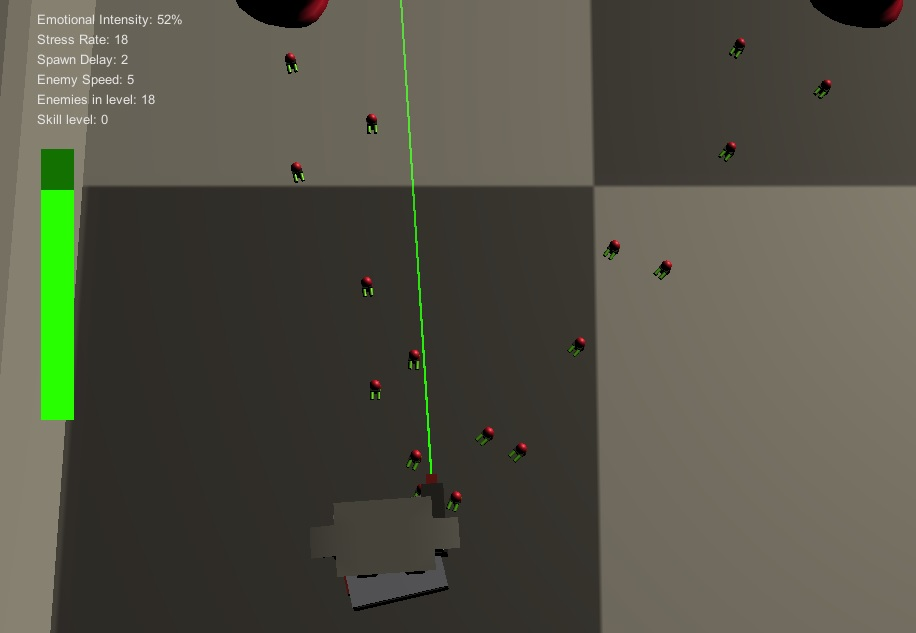
\includegraphics[width=1.0\linewidth]{artefactscreenshot.jpg}
	\caption{Screenshot of the initial prototype Artefact}
	\label{Analysis Test}
\end{figure} 

\subsection{Ethical Considerations}
There should be little to no ethical risks involved in this study. The researcher is continually referencing the British Computer Society Code of Conduct \cite{bcs} and its guidance on duty and integrity when conducting any studies and considering any ethical implications. Participants have been sampled from members of the Games Academy and were subject to the Code of Research Ethics at Falmouth University. Each participant read and agreed to a consent form (see figure 9) as well as an information sheet discussing the reasons for the study. It was stated that all participants had the right to opt-out of the study any any time without consequences and will have all the rights afforded to them as stated in the General Data Protection Regulation \cite{gdpr} if applicable, however, personal information such as name, date of birth, gender were not needed in this study. All data gathered was anonymous and confidential, with any data being stored on a secure university network drive. Participants were asked to pause the study and take a break in the unlikely event that the experiment lasted more than 30 minutes. This was to prevent any possible bouts of nausea, eye strain, or general discomfort from looking at computer screens for too long. The software was designed to account for this possibility.

\section{Artefact}
The computing artefact is a top-down 2D shooting game wherein the player defends themselves from an unending wave of zombie enemies. The following subsections describe the game in more detail.

\subsection{Basic Mechanics}
 The player has several abilities or mechanics in-built. The player has eight-directional movement using the WASD keys and can use the mouse to aim the cursor and thus aim the gun. 
The player has a cone of vision as shown in \textit{fig 4} that aims in the direction between the player character and cursor. This aiming cone shrinks and expands based on movement. The cone expands to a maximum of 25 degrees when the player moves to simulate less accuracy as is used in most first person shooters. The cone shrinks to a minimum of 5 degrees when the player is not moving or when the player 'aims down the sights' (ADS) using the right click mouse button or Left Shift, however the player movement speed is altered by a factor of 0.7, thus slowing the player and making them more vulnerable. 
The player can shoot the gun using the left click mouse button. On click, a random vector within the aiming cone field of view is chosen and a ray is cast in that direction to simulate the bullet. It takes three shots to kill an enemy when hit in a not vital area. The center of the front of the enemy is considered a vital area, therefore when the player bullet hits that weak spot the enemy is automatically killed regardless of it's remaining health. This introduces a further element of skill to the game.

\subsection{Tutorial}
The Artefact begins with the consent form displayed (see figure 9). Once the player ticks the consent icon and presses Enter, the tutorial begins. The tutorial, as seen in figure 4, has a list of objectives in the top left of the screen and contains pop-ups in the bottom center that guide the player on their current objective. 

The tutorial first teaches the players to move through a short bended corridor. Then players are taught how to shoot using stationary targets. Next the ADS mechanic is introduced and promoted as the players are given the objective to shoot the next batch of targets whilst the player is moving. These target can only be damaged if the player is moving and shooting. This is essential to teach the player since doing well at the game relies heavily on the player being able to move and shoot at the same time. Then the player moves on to the next area and has to contend with a few normal enemies that can actually attack the player in order to acclimatise the player to the basic idea of the game.

Initially, the user interface for the tutorial pop-ups were all the same colour but after pilot tests were carried out, it was noted that players did not realise the pop-ups were changing and so were not re-reading the next prompts. Therefore each time the pop-up changed, the colour scheme was changed to make it clear that new information was being given to the player. Also, the main controls were added to the top right of the tutorial to help less experienced players if they forgot the controls. 

\subsection{Main Game}
The main game level layout (see figure 3) is designed to encourage constant movement of the player. The simple placement of the 6 equally spaced out broken windows (enemy spawn areas) around the play space along with slightly different base spawn rates makes where the next enemy is coming from seem unpredictable to the player. This makes the center of the play space seem the safest to the player since they have a nearly full view of the level (see figure 20). The placement of the inner walls was used to limit line of sight and create choke points to make the game more difficult for the player and promote player movement. This has the added effect of grouping enemies chasing the player to become swarms that if left unchecked can overwhelm the player.

The various furniture objects in the level are there for aesthetic effect only and have no collision with the player or enemies. This is explained in the tutorial so as not to confuse the player. The only objects that the player collides with are the walls, broken windows and enemies.


\begin{figure}[h]
	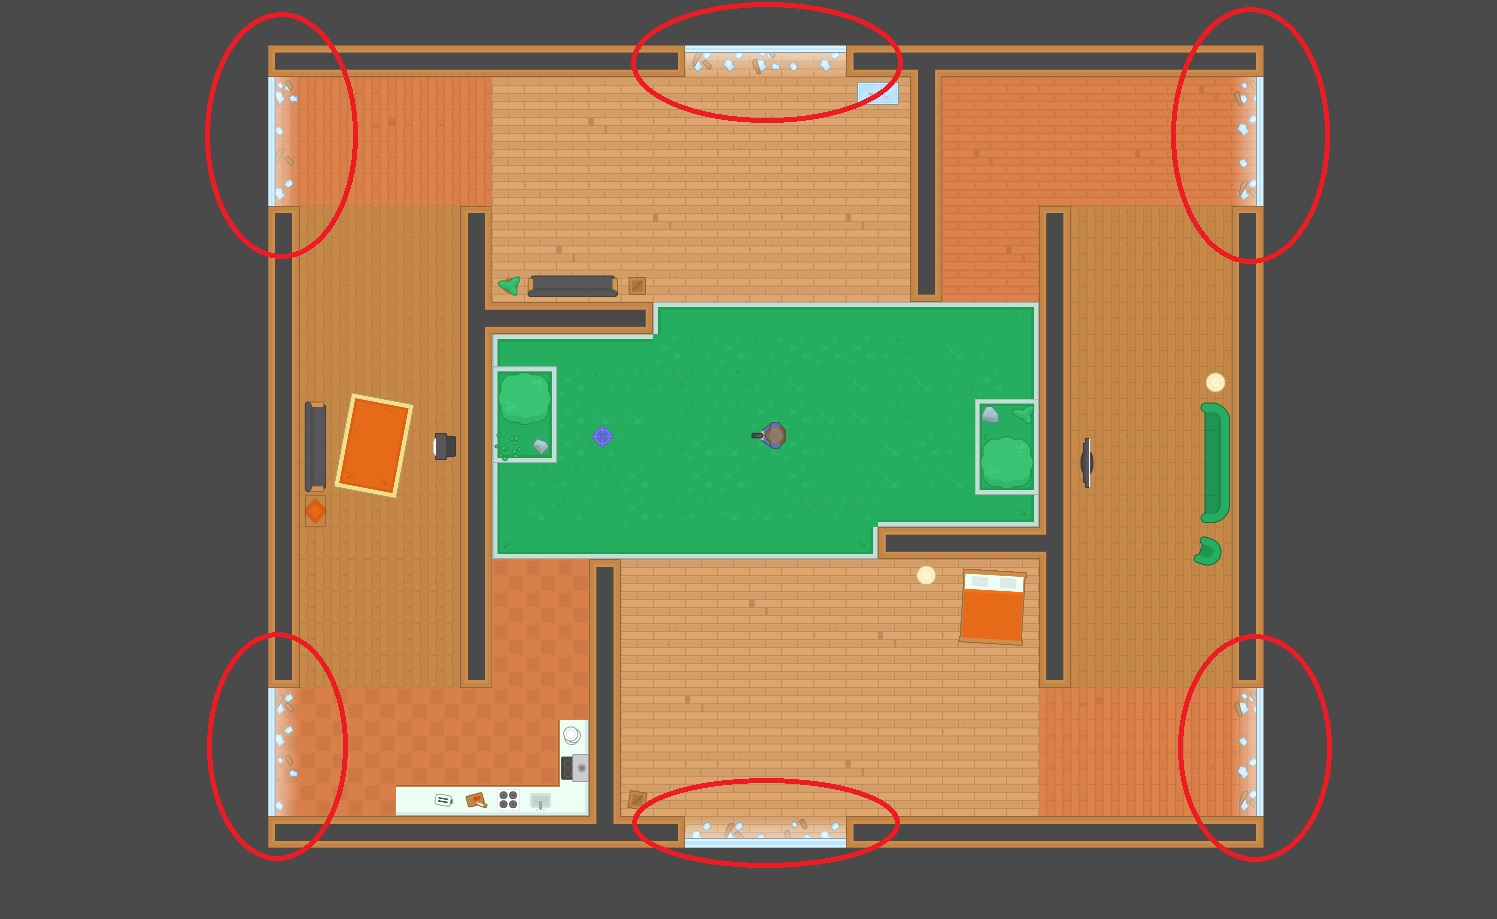
\includegraphics[width=1.0\linewidth]{artefactscreenshotlevelspawns.jpg}
	\caption{Screenshot of the Level Layout with Spawn Points Circled Red}
	\label{Analysis Test}
\end{figure} 


\begin{figure}[h]
	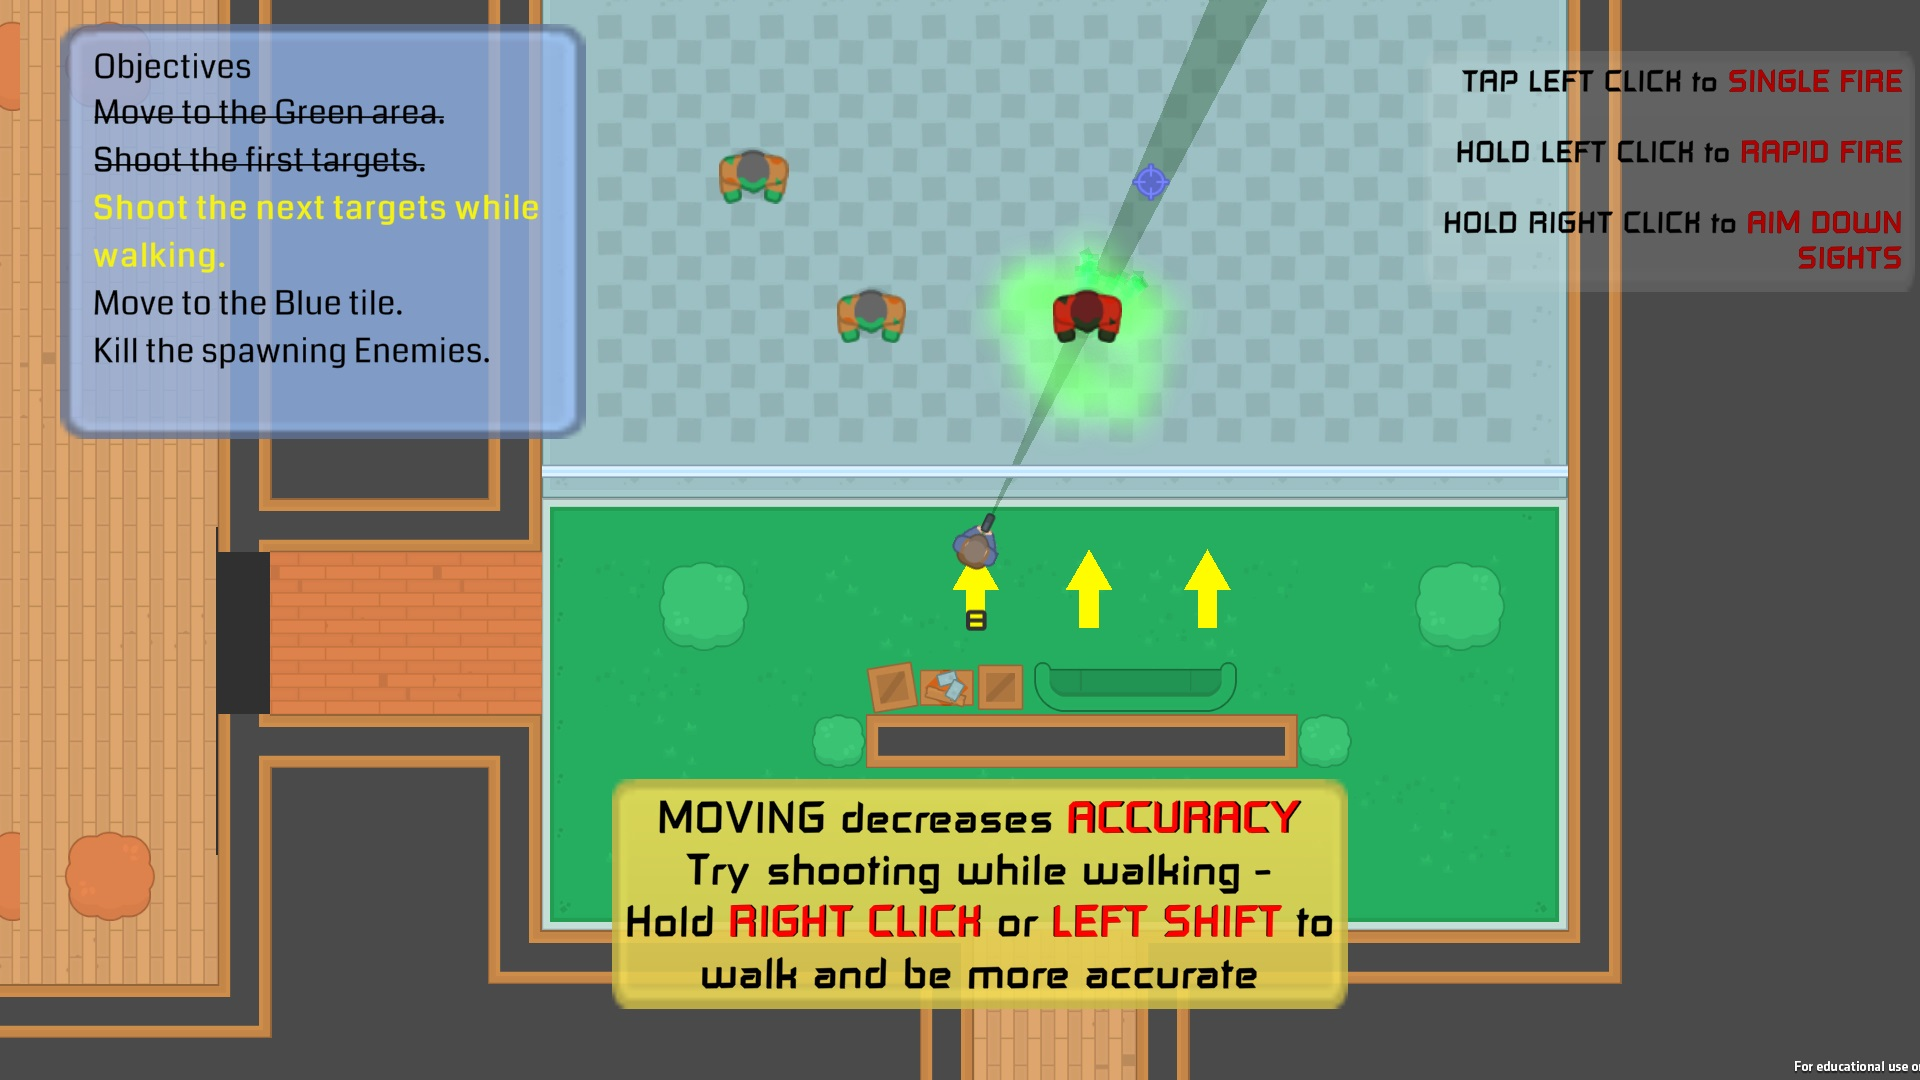
\includegraphics[width=1.0\linewidth]{tutorialscreenshot.jpg}
	\caption{Screenshot of the Tutorial}
	\label{Analysis Test}
\end{figure} 



\section{Artefact Development}

The Artefact was built using Unity 2018.4.2f1\footnote{\url{https://unity.com/}}. The DDA Algorithm was written in C\# using Visual Studio 2019\footnote{\url{https://visualstudio.microsoft.com/vs/}} as was the Top Down Shooting Game that the Algorithm would be used in. 

The enemies move using the free system ``A* Pathfinding Project\footnote{\url{https://arongranberg.com/astar/}}" found on the Unity Asset Store.

The game art was procured for free using kenney assets\footnote{\url{https://kenney.nl/assets/topdown-shooter }}. The music played during the game is called fiberitron and is a royalty free track found online\footnote{\url{https://www.dl-sounds.com/royalty-free/fiberitron-loop/}}. The sound effects used are all free sounds found online\footnote{\url{https://www.zapsplat.com/sound-effect-categories/}}.


\subsection{Dynamic Difficulty Algorithm}


Initially the plan was to use an AI Director and player grading system similar to those used in \textit{Left 4 Dead} \cite{game:left4dead} and \textit{Resident Evil 4} \cite{game:re4}. This would involve monitoring and altering heuristics as the game is being played. Originally the Artefact used a modified version of the group team game as a base. This included a twin stick player character, enemy spawners, and enemies (figure 3). A script was created called AIDirector.cs that altered spawn rates and enemy statistics such as speed, based on an emotional intensity value that ranges from 0 to 100. This value increased or decreased based on a number of factors, including but not limited to player skill, player health, number of enemies and proximity of enemies. 

During early playtesting of this system, it became clear that the complex nature of the Algorithm lead to unsatisfactory results. In other words, the game was far too simple for such a complex set of heuristics to come together and amount to desirable outcomes. Having so many factors affecting just the spawn rate and enemy speed meant that fine tuning the effect each individual heuristic had on the difficulty was very challenging. Therefore it was decided that the algorithm should be simplified. This lead to the final algorithm which is fairly simple in essence. The final design works as follows. The enemy movement speed has a value. This value is increased by a certain factor each time an enemy is killed, thus making the game more and more difficult. If the player dies, the amount by which the enemy movement speed has increased is then halved. This lowers the difficulty. If the player dies again, that increase from the base enemy speed value is halved once again, thus lowering the difficulty again. This same method is used to increase or decrease the enemy spawn rate. This is a far more simple algorithm than the previous design but works much more efficiently at simulating dynamic difficulty in order to match the skill of the player. Design adjustments were made to accommodate the new design, player health was reduced so that the player would be killed in one hit for example. This meant that it would be easier to judge player skill and challenge based on the telemetry data being gathered during testing.



\subsection{System Development Life Cycle}

The software used in this experiment was developed in it's entirety by one person. The initial prototype was created in conjunction with a video game that was in development by a team of developers including the Researcher, however, it was decided early on to discontinue this and to develop an entirely bespoke game for the project. This is mainly due to the potential risks involved in having to depend on the group based project reaching certain development milestones and not blocking the Researcher's continued development of the Artefact. Also, designing a bespoke DDA system was deemed to be much easier if the Researcher had full control of the design decisions that went into designing the game that it was to be used with. 

When developing the Artefact, the initial life cycle method proposed was the Agile Method, since team collaboration and communication would have been essential. After the decision to create a bespoke game was made, however, the development life cycle that was most suited to the project became The Prototyping Model \cite{isaias2015information}. An experimental approach to The Prototyping Model was most suited to the project since, like Agile, it is an iterative process that is more responsive to user needs. 

In order to create the Dynamic Difficulty Algorithm, the Artefact was iteratively designed and playtests were conducted throughout development in order to validate and verify it \cite{fullerton2004game}. Therefore it was ensured that anyone who playtested throughout development was not in the final experiment, since this may have biased the results. It was decided early on that creating an Artificial Intelligence (AI) agent would be more beneficial and more efficient than gathering playtesters constantly throughout development and so a Player AI was designed for testing purposes.

The user needs, such as the flow of the game and the effectiveness of the DDA Algorithm could be proposed and evaluated through pilot testing and AI simulations. Then once feedback is attained, the system could be refined to attempt to improve and revise the Prototype to then be tested again until the Prototype satisfies all user requirements.

\subsection{Software Testing}

The DDA Algorithm functionality was tested using a combination of pilot testing and a Player Artificial Intelligence Agent that simulates the player. Initially, each iteration of the Artefact was to be tested using human players. However, this seemed to be an impractical method of testing the DDA Algorithm. The development of a working dynamic difficulty system requires many refinements and iterations to be tested, which would mean a lot of participants would be required to do pilot tests throughout development. There are ways of limiting the impracticality of this, such as with posting the Artefact online to get feedback from players, on the other hand, these methods also come with drawbacks and would likely slow development considerably while waiting for feedback. Thus, a Player AI was developed to simulate the player so that testing of the DDA Algorithm could be much faster. 

The Player AI has fairly basic pathfinding abilities and as such cannot be said to be as human-like as can be but serves the purposes of testing the difficulty system. The Player AI moves between the four corners of the map using the same A* Pathfinding that the enemies in the game use. The Player AI will interrupt it's pathfinding and move away from enemies that get too close however, somewhat simulating a human player. The Player AI has most of the same systems as the Player Prefab in-game. To adjust the Skill Level of the Player AI, the shots per second and accuracy values can be adjusted. As the player has an accuracy cone system built into the design, the Player AI uses this when aiming at the nearest enemy with a clear line of sight and therefore the Skill Level of the AI can be adjusted by adjusting the spread of this cone, thus adjusting the shot accuracy of the AI. Pilot tests were carried out to assess the Player AI against human players and adjust the shots per second and accuracy values in order to get as accurate a representation of human gameplay as possible. A static difficulty curve with an unchanging spawn rate was used in the pilot test. The average Kill/Death Ratios (KDR) of the five pilot testers was used as a base to aim towards when adjusting the shot accuracy and shooting rate of the Player AI. When the Player AI had achieved a similar enough KDR in simulations with the same static difficulty, it was deemed as being satisfactorily functional for the purposes of testing the DDA Algorithm.

\section{Results and Analysis}

The data gathered from the experiment were output into a csv file on the university network drive. RStudio 1.2.5019\footnote{\url{https://rstudio.com/products/rstudio/download/}} was used to collate and process the results. The R package ggplot2 was used to generate the graphs.

\subsection{Hypothesis 1 - Players will enjoy playing the version with dynamic difficulty more than the version with static difficulty}

This hypothesis was intended to judge whether or not players enjoyed playing the dynamic version of the game over the static version. Figure 6 shows us that there is a slight preference for the dynamic version. A t-test was carried out analysing the differences in how the players scored the two difficulty versions on the basis of player enjoyment. This test produced a p-value of 0.001638 and a t-value of 3.0634. The p-value is very low and therefore the null hypothesis can be rejected. The mean value of the differences was 6.08 showing that on average players enjoyed the dynamic version 6 percent more than the static version.


\begin{figure}[h]
	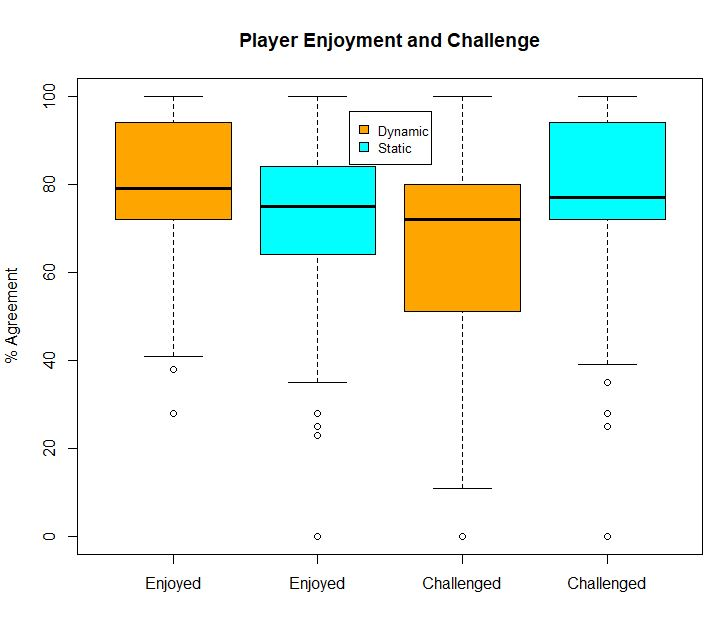
\includegraphics[width=1.0\linewidth]{playerenjoymentandchallenge.jpg}
	\caption{Boxplot of Enjoyment and Challenge Perceptions}
	\label{Analysis Test}
\end{figure} 

\begin{figure*}[h]
	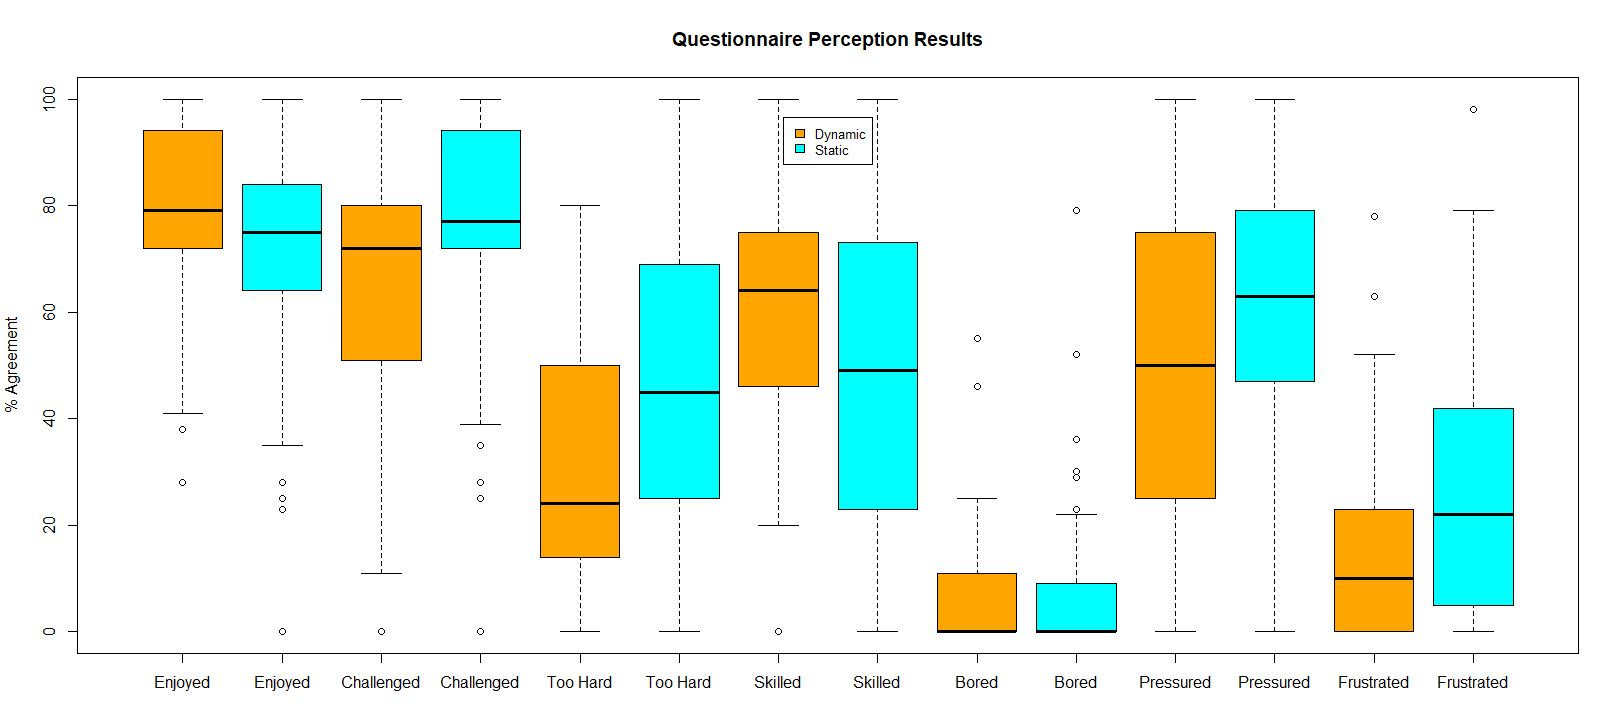
\includegraphics[width=1.0\linewidth]{questionnaireboxplot.jpg}
	\caption{How Players Felt Playing Each Difficulty System}
	\label{Analysis Test}
\end{figure*} 





\subsection{Hypothesis 2 - There will be more variation in how challenged players were playing with static difficulty than when playing with dynamic difficulty}

An F-Test was carried out to determine the variance of player deaths between the two difficulty versions. This is deemed by the researcher to be a valid assessment of difficulty. The test produced a p-value of 2.277e-09. This p-value is extremely low and therefore the null hypothesis can be rejected. The ratio of variances was 4.9226.

Interestingly, player perception of difficulty may not be as varied as can be seen in Figure 11.  Therefore a second F-Test was carried out in order to determine the variance in challenge scores the two difficulty versions received by each player. This test analyses player perception of difficulty and therefore is tangentially related to the hypothesis in question. This second test produced a p-value of 0.4927. This p-value is too high and therefore the null hypothesis would not be rejected. The ratio of variances was 1.0047.

This seems to indicate that although the difficulty appears to be more varied based on player deaths with the static difficulty, the perception of difficulty among players is less varied than one would expect.



\subsection{Hypothesis 3 - Players will be unable to reliably judge which version used dynamic difficulty}

The data showed that 36 out of the 61 participants in the study correctly guessed which level used the dynamic difficulty system. A Chi-squared test was performed to determine the probability that this was higher that random chance. The test produced a p-value of 0.159. This p-value is low enough to discount the null hypothesis. This suggests that players were not able to reliably identify which version used dynamic difficulty.



\begin{figure}[h]
	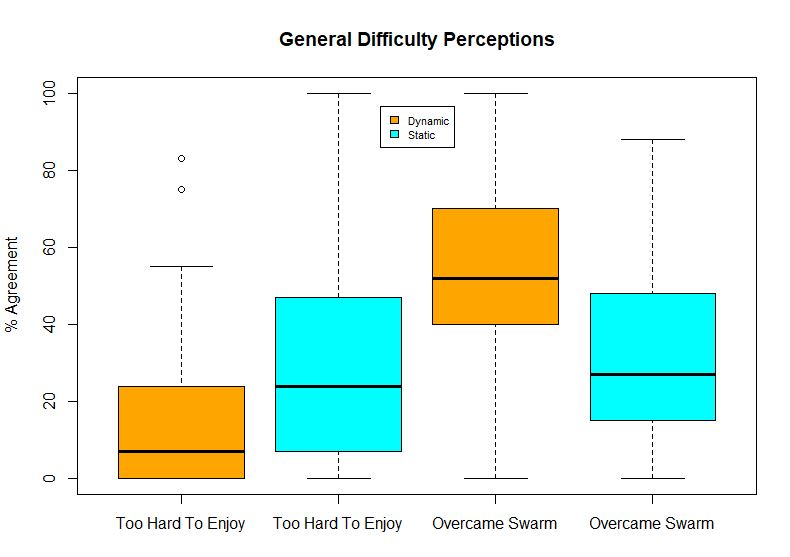
\includegraphics[width=1.0\linewidth]{difficultyperceptions.jpg}
	\caption{Boxplot of Challenge Perceptions}
	\label{Analysis Test}
\end{figure} 

\section{Discussion}
The results from this experiment suggest that player enjoyment and challenge is affected by a games difficulty system. Although not drastically different, as shown in figure 5, the evidence suggests that the dynamic difficulty as implemented in this particular experiment was more enjoyable and less challenging to players than the static difficulty. The potential reasons behind this are discussed in this section.

As you can see from the findings illustrated in figure 6, on average players found the dynamic version more enjoyable than the static version. This is a fairly small difference but since the difficulty system is the only thing that was changed between the two levels, it's still a significant difference. The findings also show that players generally didn't get bored playing either version. 

The static version could become too hard for some players to enjoy whereas the dynamic version suffered from this problem less. Evidence that this could be the case can be seen in figure 7. This may indicate that the dynamic algorithm is functioning correctly in adapting challenge to player skill. The alternative could be that the static version was just designed to be too difficult for most players despite the researcher using the pilot tests to verify the overall difficulty of the static version.

The game would allow up to 15 enemies on the screen at a time if players could not defeat them fast enough, this could lead to a swarm of enemies attacking the player at times. As shown in figure 7, these swarms were more likely to be overcome by the player in the dynamic version. This is likely due to the fact that enemy speed values would be lowered if the player is struggling in the dynamic version whereas in the static version the enemy speed and spawn rate steadily increases regardless of the skill of the individual player. The ability of the player to overcome adversity is a possible factor in how much they enjoyed the game and how difficult it felt for them.

In figure 15 we can see that with the dynamic version, there is a very slight positive correlation between how skilled players felt and how challenged they felt. The opposite can be seen with the static version in figure 16 where it seems that the more skilled a player felt, the less challenging the game felt. This is an interesting observation and could suggest that when a difficulty system is dynamic, the player is more likely to feel like they are good at the game despite feeling that the game is challenging to them or perhaps even because the game is challenging them appropriately for how good they are.

Figure 6 also shows that with the dynamic version, players never felt bored and rarely felt frustrated. This, coupled with the fact players did feel challenged and similarly skilled, promotes the idea that the dynamic version successfully achieved ''Game Flow" as discussed previously and in figure 1. This cannot be said for the static version since although not feeling bored, more players felt frustrated and there was much more disparity between how challenged they felt and how skilled they felt. 




\section{Limitations}

Although it is particularly encouraging to see that the results in figure 6 reflect the idea that the dynamic version indeed created flow, it cannot be forgotten that flow is particularly difficult to quantify and correctly assess. This is especially true with a game as short as the game in this experiment.

It must be noted that one player decided to go against the objective of killing as many enemies as possible and just outrun the enemies in the dynamic version of the game. Since the enemies were not being killed and there was a limit of 15 enemies spawned at a time, the player was able to outrun the enemies for the whole 150 seconds without dying. This is a design flaw in the algorithm the researcher did not foresee. It should be noted that this player was a professional game designer and the data from this player was omitted from the rest of the results since it would not be fairly judging the algorithm as it's intended to work. To correct this, the algorithm could be adjusted to increase the difficulty when a stalemate like this occurs.

\section{Further Research}
As stated in the limitations section above, there are many things that could be studied further to gain insight into how dynamic difficulty can affect player enjoyment and challenge. 

Player experience and game flow are particularly hard to quantify and assess in such a small scoped experiment. A more lengthy study on a game with a longer experiment time would be ideal. Since most commercial games can last several hours, it is important to be able to conduct more experiments on dynamic difficulty in a controlled manner on a much larger scale than was done in this study. The levels in this study only lasted two and a half minutes each and so cannot replicate the experience created by most commercial games today. It would be interesting to see how bigger games with more content would be affected by dynamic difficulty compared with standard static difficulty systems. 

% references section

\bibliographystyle{IEEEtran}
\bibliography{references}

% Appendices

\appendices
\section{Acknowledgements}
I would like to thank all of the staff at Falmouth University for their help and support, particularly on the BSc Computing for Games Course. I would also like to thank my dissertation supervisor Brian McDonald for keeping us students on track. Many thanks also to my fellow university students for their help with playtesting and dissertation feedback.

\section{Reflective Report}
The following subsections will discuss the various issues I have encountered during the development of this dissertation. Each issue will declare a SMART goal that can be actioned upon to help better myself in those areas.

\subsection{Artefact Verification}

\subsection{Approaching Participants}

\subsection{Level Design}

\subsection{Time Management}

\subsection{Motivation}

\section{Additional Materials}

Link to Repository:
\url{https://gamesgit.falmouth.ac.uk/scm/~ac200905/dda_artefact.git}

The specific script I have made for the Dynamic Difficulty Algorithm is AIDirector.cs but the entirety of the Unity Project was created and designed for the experiment.

\subsection{Unit Tests}
Figure 13 shows the unit tests created for the AIDirector using the Unity Test Runner.

\begin{figure}[h]
	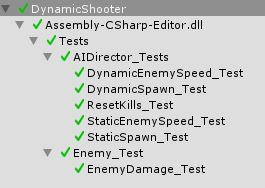
\includegraphics[width=1.0\linewidth]{unittests.jpg}
	\caption{Static Scatter plot of Player Enjoyment vs Player Deaths}
	\label{Analysis Test}
\end{figure}

\begin{figure*}[h]
	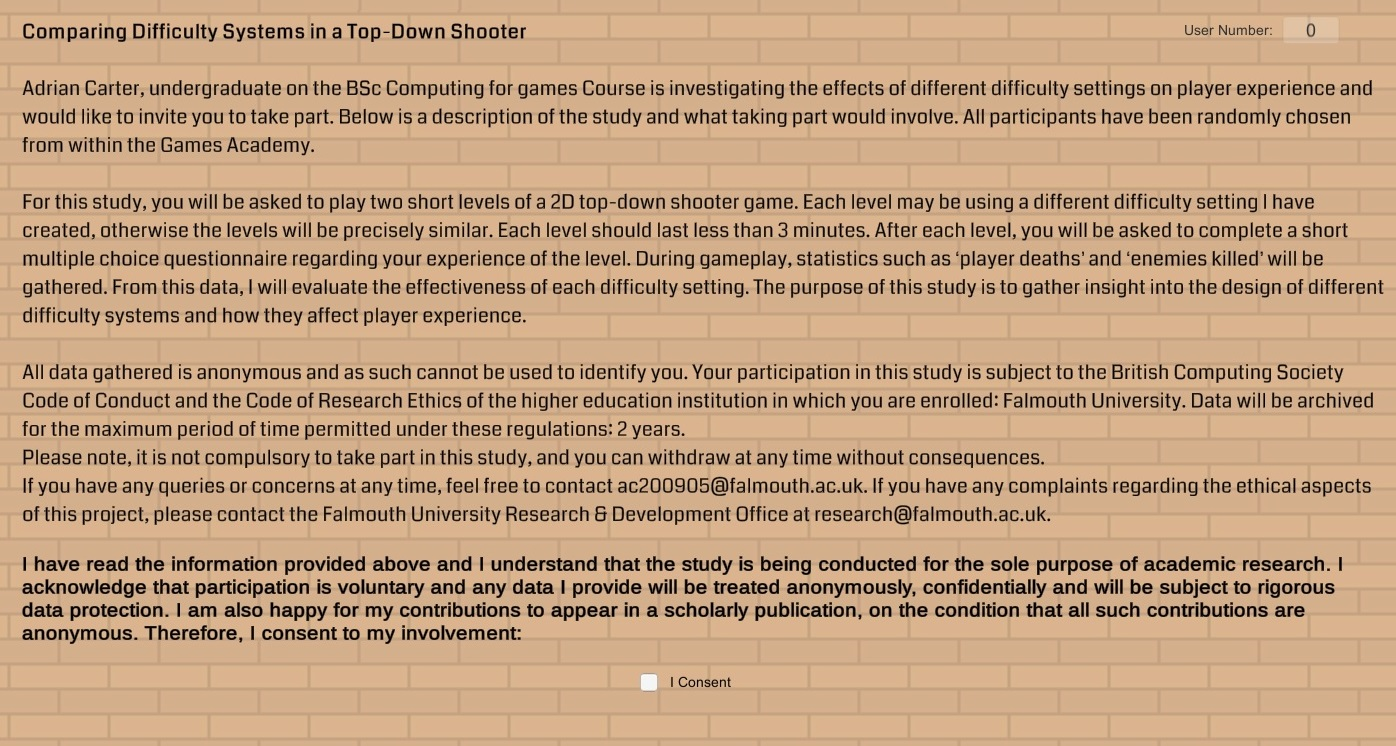
\includegraphics[width=0.75\linewidth]{consentformingame.jpg}
	\caption{Consent Form}
	\label{Analysis Test}
\end{figure*} 

\begin{figure*}[h]
	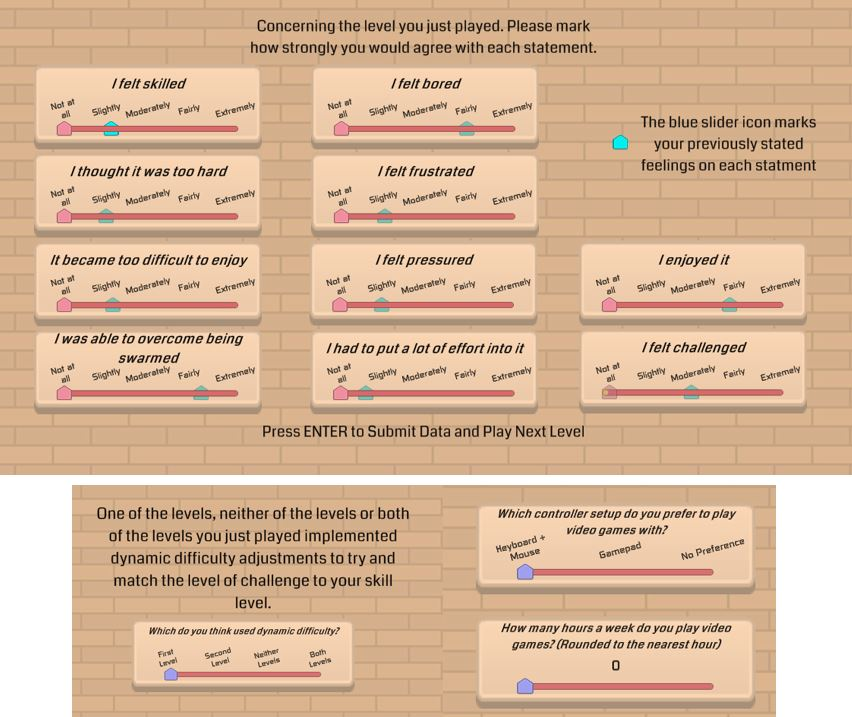
\includegraphics[width=0.75\linewidth]{questionnaireingame.jpg}
	\caption{In-Game Questionnaire}
	\label{Analysis Test}
\end{figure*} 



Figure 14 shows the final iteration of the consent form. While originally it was designed to be in paper form, it was decided that implementing it into the beginning of the artefact itself would be more efficient and enables the participant to consent before even being able to access the game.

\begin{figure*}[h]
	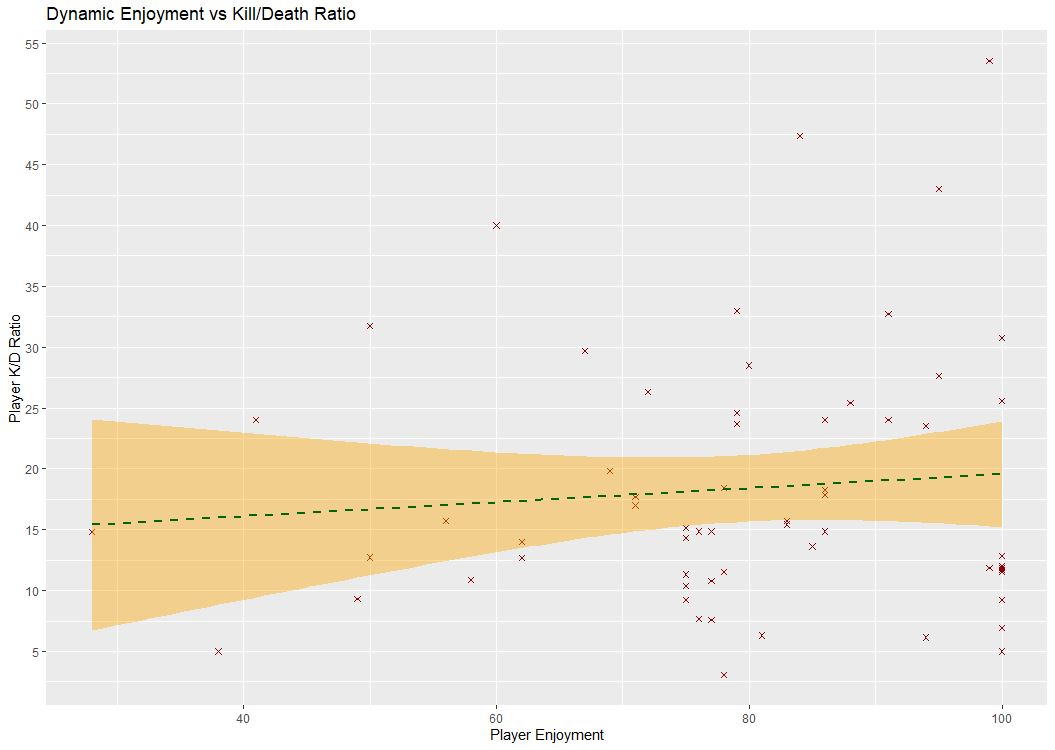
\includegraphics[width=0.75\linewidth]{dynamicfunKDR.jpg}
	\caption{Scatter plot of Player Enjoyment vs Player Kill/Death Ratio}
	\label{Analysis Test}
\end{figure*} 

\begin{figure*}[h]
	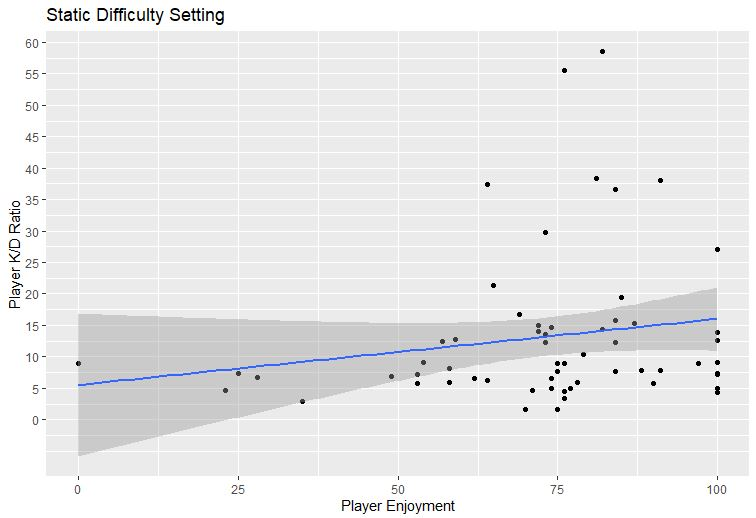
\includegraphics[width=0.75\linewidth]{staticfunKDR.jpg}
	\caption{Static Scatter plot of Player Enjoyment vs Player Kill/Death Ratio}
	\label{Analysis Test}
\end{figure*} 

\begin{figure*}[h]
	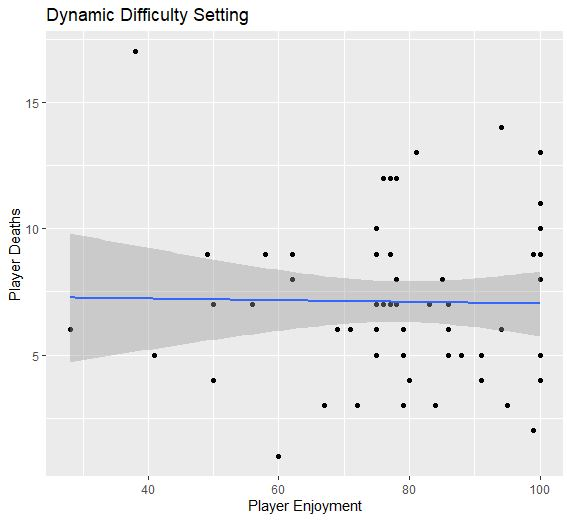
\includegraphics[width=0.75\linewidth]{dynamicfundeath.jpg}
	\caption{Dynamic Scatter plot of Player Enjoyment vs Player Deaths}
	\label{Analysis Test}
\end{figure*} 

\begin{figure*}[h]
	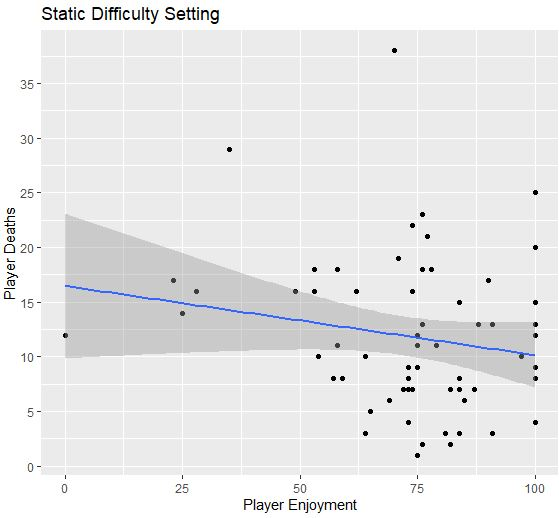
\includegraphics[width=0.75\linewidth]{staticfundeath.jpg}
	\caption{Static Scatter plot of Player Enjoyment vs Player Deaths}
	\label{Analysis Test}
\end{figure*}

\begin{figure*}[h]
	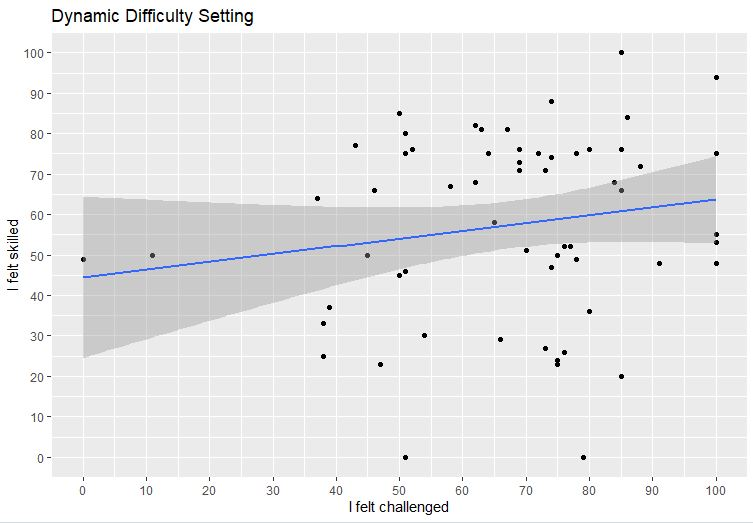
\includegraphics[width=0.75\linewidth]{dynamicchallengevsskilled.jpg}
	\caption{Dynamic Scatter plot of Skill and Challenge Perceptions}
	\label{Analysis Test}
\end{figure*} 

\begin{figure*}[h]
	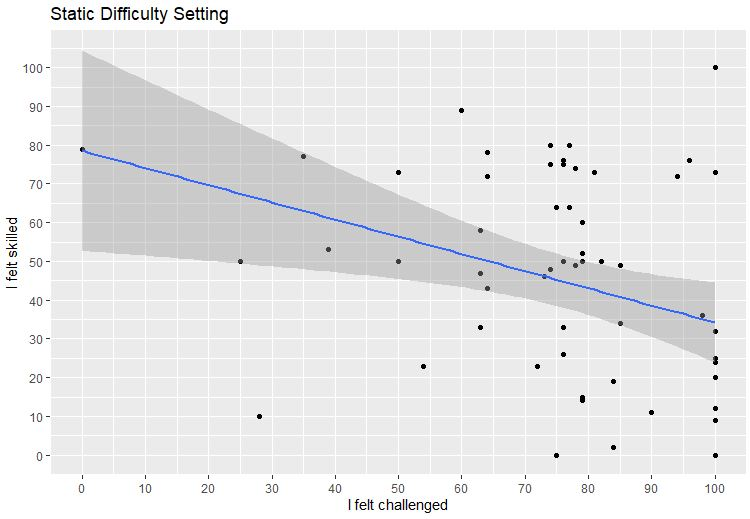
\includegraphics[width=0.75\linewidth]{staticchallengevsskilled.jpg}
	\caption{Static Scatter plot of Skill and Challenge Perceptions}
	\label{Analysis Test}
\end{figure*} 

\begin{figure*}[h]
	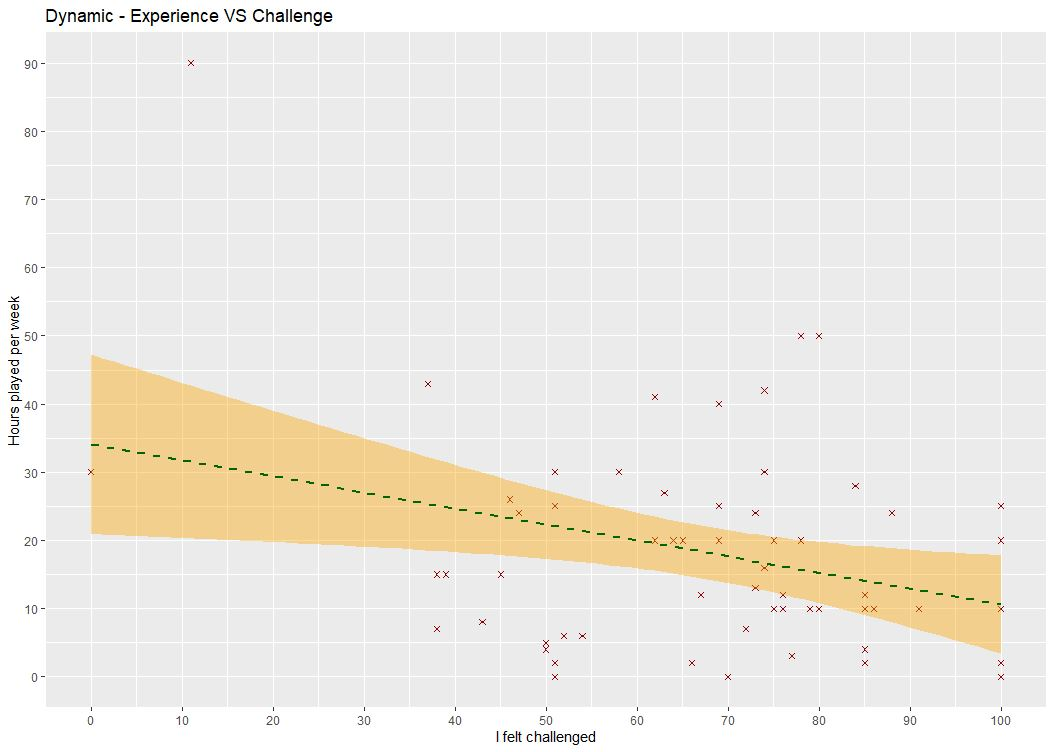
\includegraphics[width=0.75\linewidth]{dynamicexpvschallenge.jpg}
	\caption{Dynamic Scatter plot of Experience and Challenge Perceptions}
	\label{Analysis Test}
\end{figure*}

\begin{figure*}[h]
	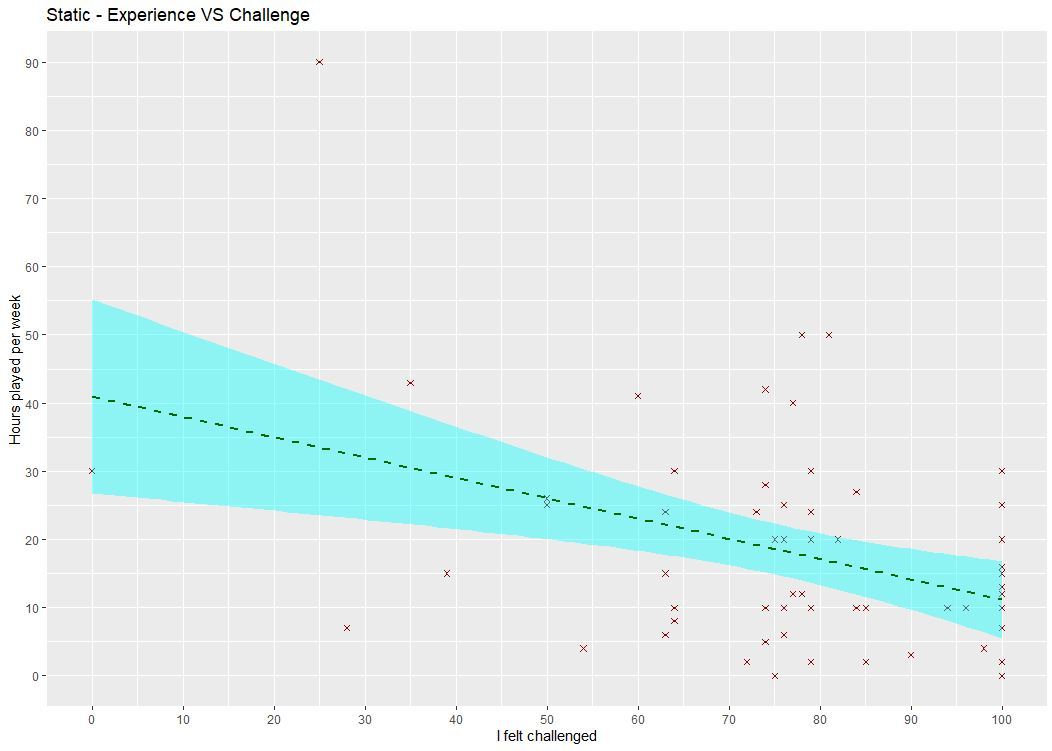
\includegraphics[width=0.75\linewidth]{staticexpvschallenge.jpg}
	\caption{Static Scatter plot of Experience and Challenge Perceptions}
	\label{Analysis Test}
\end{figure*}

\begin{figure*}[h]
	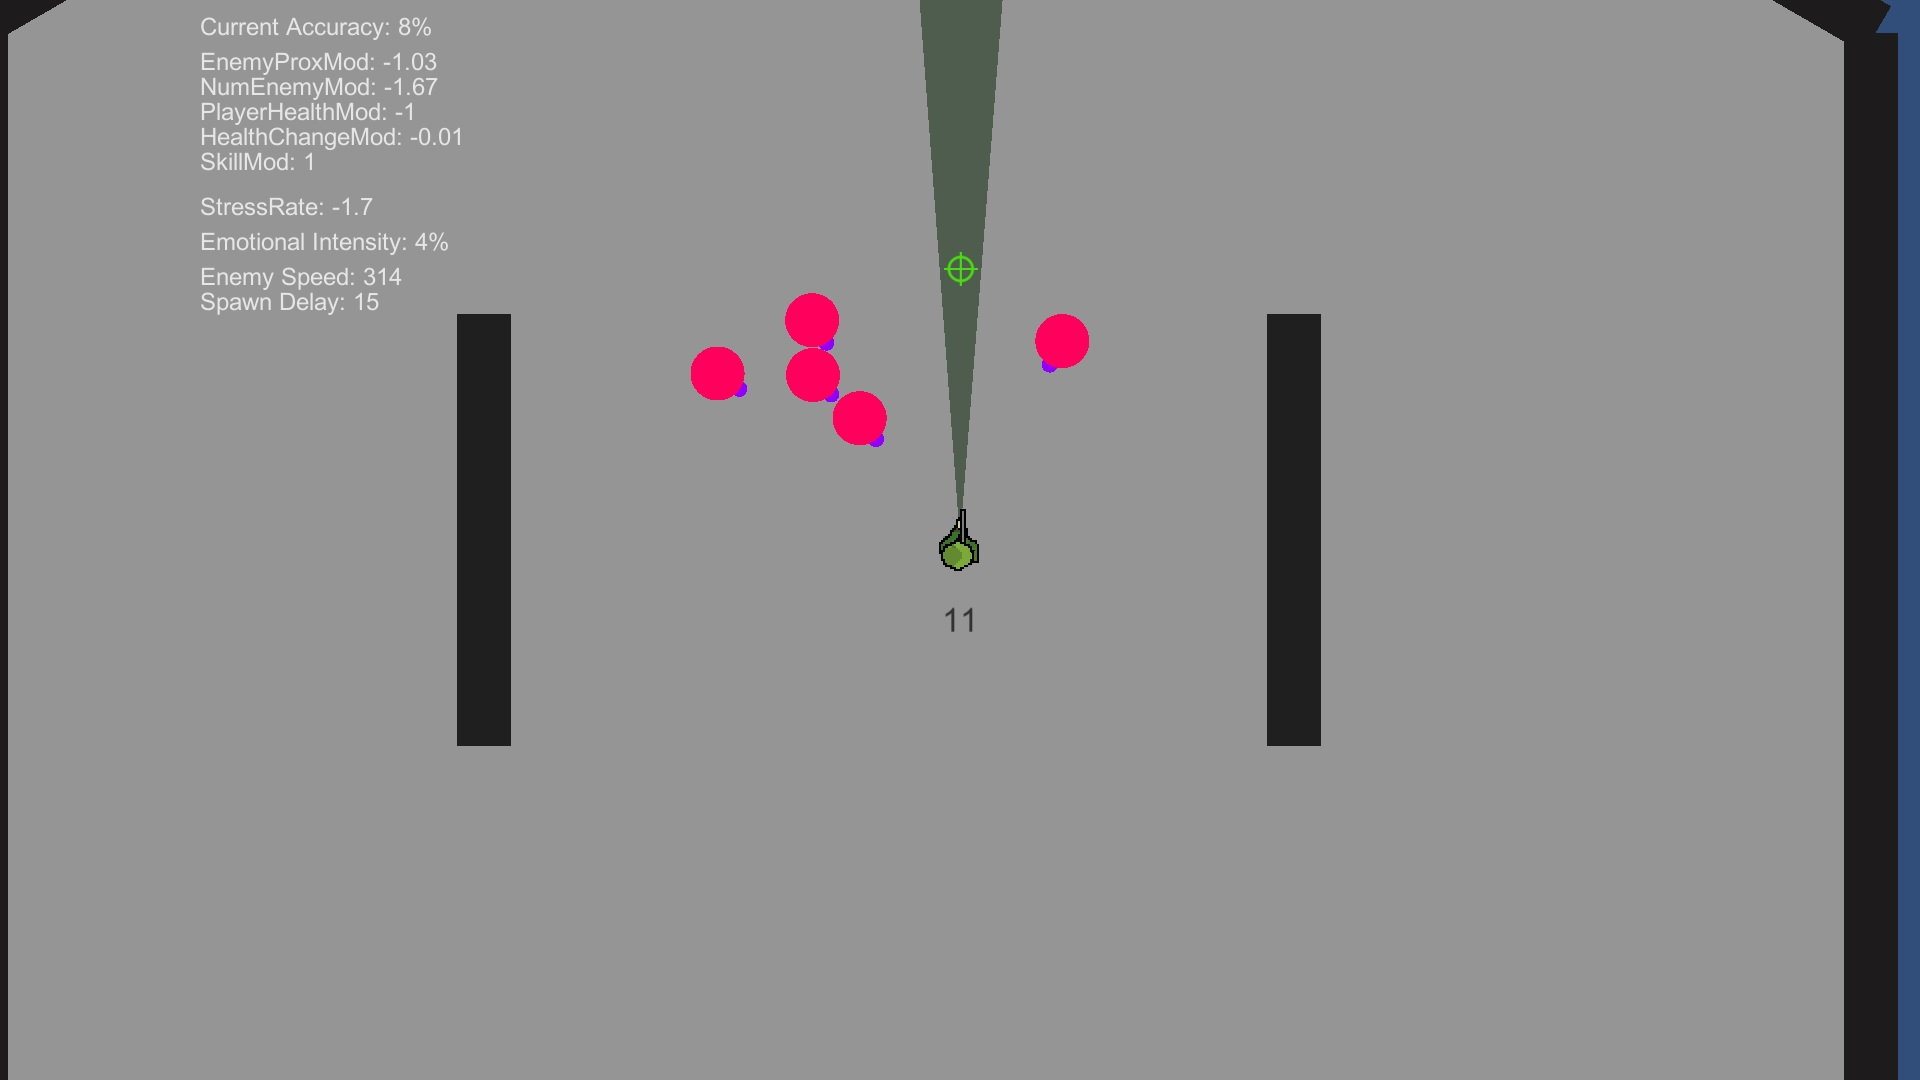
\includegraphics[width=0.75\linewidth]{secondprototype.jpg}
	\caption{Initial Bespoke Game Prototype}
	\label{Analysis Test}
\end{figure*} 

\begin{figure*}[h]
	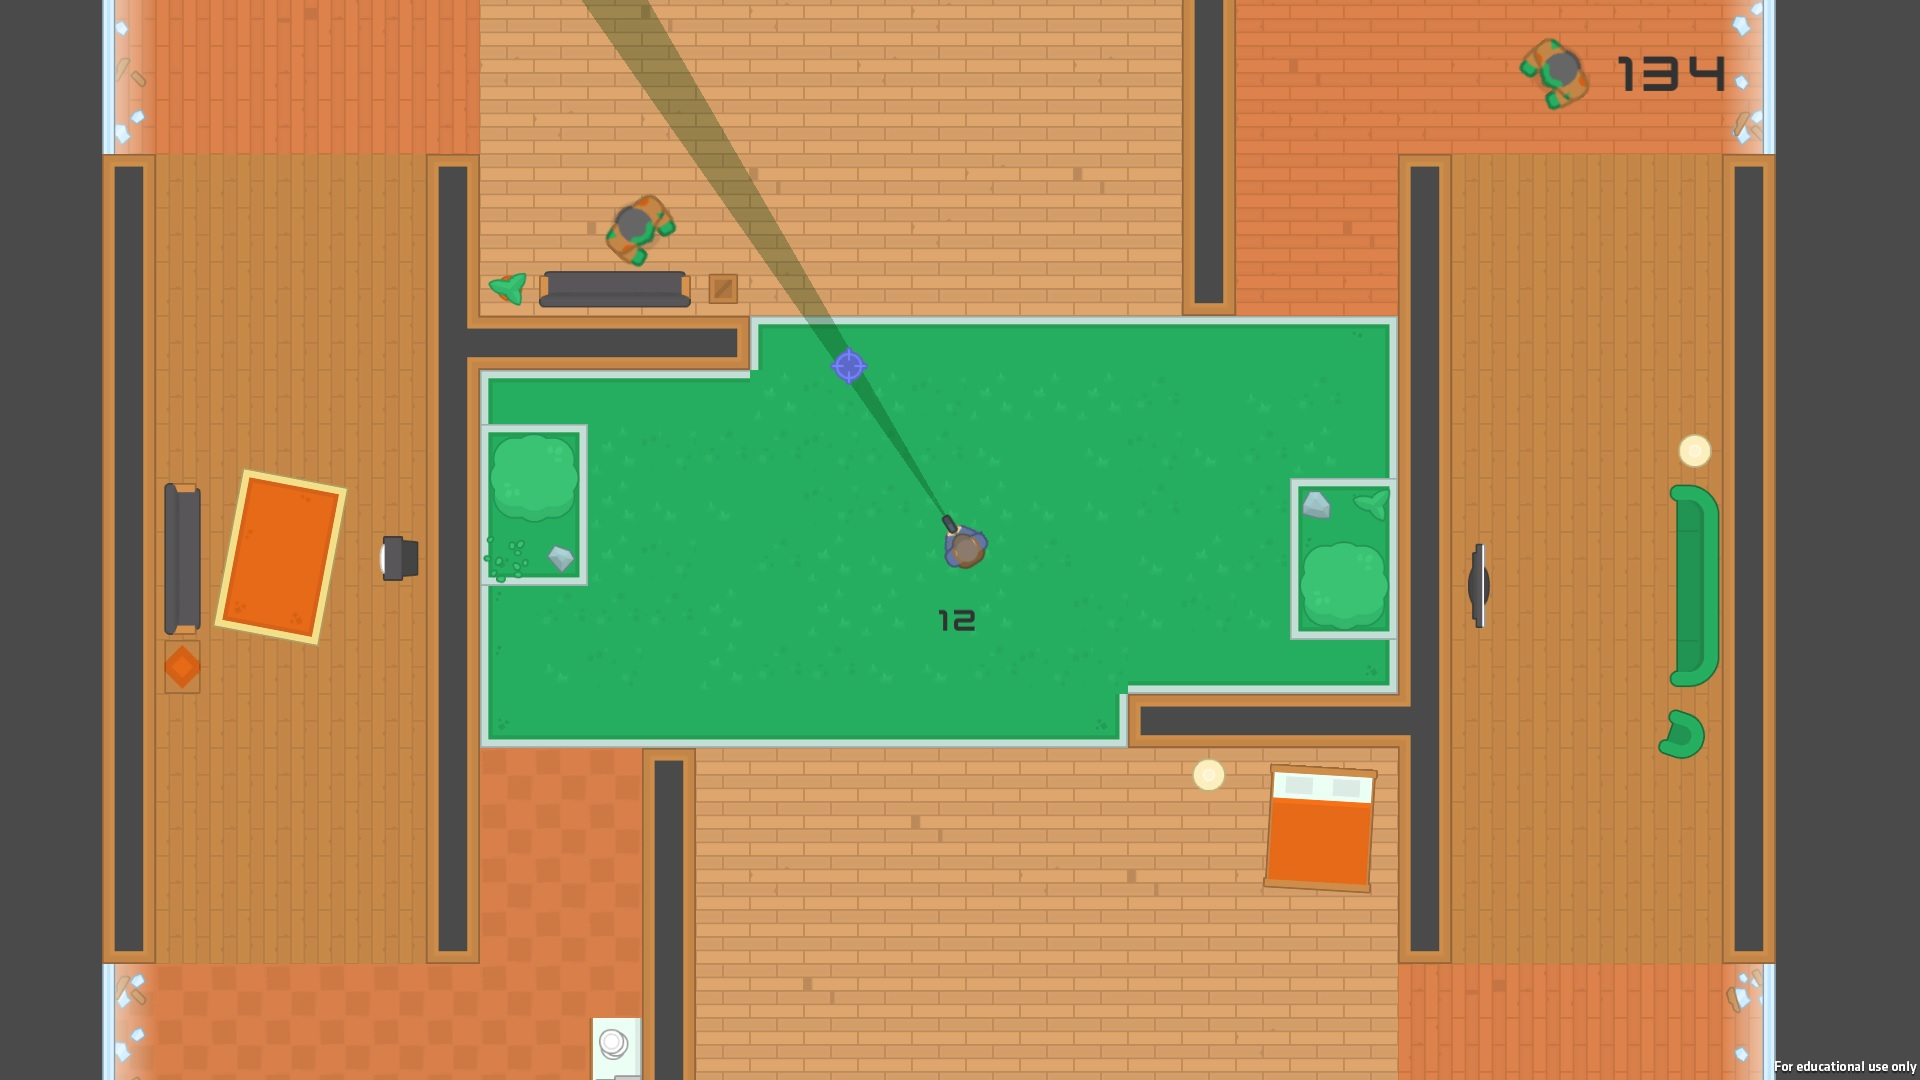
\includegraphics[width=0.75\linewidth]{maingame.jpg}
	\caption{Screenshot of the Main Game Level}
	\label{Analysis Test}
\end{figure*} 


\begin{center}
\begin{figure*}


\begin{lstlisting}[language=R]

#install.packages("readr")
#install.packages("psych")

library(readr)
library(ggplot2)

# Find CSV data set and import it
dat <-read.csv("D:/user_data.csv")

# T-Test for Hypothesis 1 -----------
# Testing to see if players enjoyed the dynamic version more than the static
funTest <- t.test(dat$FunScoresDynamic,dat$FunScoresStatic,paired=TRUE, alternative="greater")

# If not normally distributed - paired dependent
funTest <- wilcox.test(dat$FunScoresDynamic,dat$FunScoresStatic, paired = TRUE,  alternative="greater")

funTest$p.value
funTest$estimate

# Check if normal distribution
ggplot(data=dat, aes(dat$StaticEnjoyed)) + 
+     geom_histogram(breaks=seq(0, 100, by=1))

# F-Test for Hypothesis 2 ------------
# Testing to see if the variances of player deaths in static version is higher than the 
# variance in player deaths in the dynamic version
challengeTest <- var.test(dat$Static.Deaths, dat$Dynamic.Deaths, alternative = "greater")

# Testing to see if the variances of player challenge scores in static version is higher than 
# the variance in player challenge scores in the dynamic version
challengeTest2 <- var.test(dat$ChallengeScoresStatic, dat$ChallengeScoresDynamic, alternative
= "greater")

# Chi-Square Test for Hypothesis 3 ---------
correctVsIncorrect < c(numCorrect, numIncorrect)

# Chi square test to see if players guessed the dynamic version correctly more significantly
# often than by random chance
# If the p-values is smaller than 0.05 then the player guesses are significantly not commonly
# distributed between correct and incorrect, thus meaning one is significantly higher and a
# further test needs to be made to see if it is the correct answer
versionChoiceRandomTest <- chisq.test(correctVsIncorrect, p = c(1/2, 1/2))

# If answers were not given at the rate of random chance, were answers more often correct?
versionChoiceCorrectTest <- chisq.test(correctVsIncorrect, p = c(4/5, 1/5))


# For pilot tests ---------
pilotKDTest <- t.test(dat$EnemiesKilledStatic, y, paired = TRUE, alternative = "two.sided")

# Use this scatter graph to see if Kill/Death Ratios are similar between players using the
# dynamic setting
ggplot(dat, aes(x=dat$PlayerKDRatioDynamic, y=dat$PlayerKDRatioDynamic)) + geom_point() 
+ geom_smooth(method=lm)


\end{lstlisting}

\end{figure*}

\end{center} 
 
 
\begin{center}
\begin{figure*}


\begin{lstlisting}[language=R]


# Graphs to look for correlations in the data I will be collecting

# Box plot showing the differences in fun between both difficulty settings
boxplot(dat$FunScoresDynamic, dat$FunScoresStatic)

# Box plot showing the differences in challenge between both difficulty settings
boxplot(dat$ChallengeScoresDynamic, dat$ChallengeScoresStatic)

# Fun and Challenge together
boxplot(dat$FunScoresDynamic, dat$FunScoresStatic, 

dat$ChallengeScoresDynamic, dat$ChallengeScoresStatic,
names = c("Enjoyed", "Enjoyed", 

"Challenged", "Challenged" ), 
main = "Player Enjoyment and Challenge", col=(c("orange","cyan")), 
ylab = "% Agreement")
legend("top", inset=.07, cex=0.8, legend = c("Dynamic","Static") , 
col = c("orange", "cyan"), fill = c("orange", "cyan"))


# Boxplot with both challenge and fun
boxplot(dat$ChallengeScoresDynamic, dat$ChallengeScoresStatic, 
dat$FunScoresDynamic, dat$FunScoresStatic, 
names = c("Dynamic Challenge", "Static Challenge", "Dynamic Fun",  
"Static Fun"), 
main = "Comparing Fun and Challenge", col=(c("orange","cyan")), 
ylab = "% Agreement")

# Boredom and frustration comparisons
boxplot(dat$Dynamic...I.felt.bored, dat$Static...I.felt.bored, 
dat$Dynamic...I.felt.frustrated, dat$Static...I.felt.frustrated, 
names = c("Dynamic Boredom", "Static Boredom", "Dynamic Frustration",  
"Static Frustration"), 
main = "Comparing Boredom and Frustration", col=(c("orange","cyan")), 
ylab = "% Agreement")

# Boxplot for 'Too hard to enjoy' and 'overcame being swarmed'
boxplot(dat$Dynamic...It.became.too.difficult.to.enjoy, 
dat$Static...It.became.too.difficult.to.enjoy, 
dat$Dynamic...I.was.able.to.overcome.being.swarmed, 
dat$Static...I.was.able.to.overcome.being.swarmed,
names = c("Too Hard To Enjoy", "Too Hard To Enjoy", 
"Overcame Swarm", "Overcame Swarm" ), 
main = "General Difficulty Perceptions", col=(c("orange","cyan")), 
ylab = "% Agreement")

legend("top", inset=.07, cex=0.8, legend = c("Dynamic","Static") , 
col = c("orange", "cyan"), fill = c("orange", "cyan"))



\end{lstlisting}

\end{figure*}

\end{center}




\begin{center}
\begin{figure*}


\begin{lstlisting}[language=R]
# Boxplot of Questionnaire Results
boxplot(dat$FunScoresDynamic, dat$FunScoresStatic,
dat$ChallengeScoresDynamic, dat$ChallengeScoresStatic,
dat$Dynamic...I.thought.it.was.too.hard, 
dat$Static...I.thought.it.was.too.hard, 
dat$Dynamic...I.felt.skilled, dat$Static...I.felt.skilled,
dat$Dynamic...I.felt.bored, dat$Static...I.felt.bored,
dat$Dynamic...I.felt.pressured, dat$Static...I.felt.pressured,
dat$Dynamic...I.felt.frustrated, dat$Static...I.felt.frustrated,
names = c("Enjoyed", "Enjoyed",
"Challenged", "Challenged",
"Too Hard", "Too Hard", 
"Skilled", "Skilled",
"Bored", "Bored",
"Pressured", "Pressured",
"Frustrated", "Frustrated"), 
main = "Questionnaire Perception Results", col=(c("orange","cyan")), 
ylab = "% Agreement")

legend("top", inset=.07, cex=0.8, legend = c("Dynamic","Static") , 
col = c("orange", "cyan"), fill = c("orange", "cyan"))

# Examples of scatter graph R code -------------------

# Scatter graph with line of best fit to see if the more a player 
# dies the less they enjoyed the game
ggplot(dat, aes(x=FunScoresDynamic, y=PlayerDeathsStatic)) + geom_point() +
geom_smooth(method=lm)

# Dynamic - Player Deaths vs enjoyment
ggplot(dat, aes(x=FunScoresDynamic, y=Dynamic.Deaths)) + 
geom_point(shape=4, color="darkred") + 
geom_smooth(method=lm, linetype="dashed",
color="darkgreen", fill="orange") +
xlab("Player Enjoyment") + ylab("Player Deaths") + 
ggtitle("Dynamic Enjoyment vs Deaths") + 
scale_y_continuous(breaks = c(0,5,10,15,20,25,30,35,40))

# Static - Player Deaths vs enjoyment
ggplot(dat, aes(x=FunScoresStatic, y=Static.Deaths)) + 
geom_point(shape=4, color="darkred") + 
geom_smooth(method=lm, linetype="dashed",
             color="darkgreen", fill="cyan") +
xlab("Player Enjoyment") + ylab("Player Deaths") +
 ggtitle("Static Enjoyment vs Deaths") + 
scale_y_continuous(breaks = c(0,5,10,15,20,25,30,35,40))

\end{lstlisting}

\end{figure*}

\end{center}






% that's all folks
\end{document}
